\documentclass[a4paper]{article}

\usepackage[inline]{enumitem}

\newlist{inl}{enumerate*}{1}
\setlist[inl]{
    label=\mbox{\rm($\roman*$)},
}

\usepackage{tabularx}

\usepackage{float}
\usepackage[small]{caption}

\usepackage[citestyle=numeric-comp,
    giveninits,doi=false,url=false,
    natbib,sortcites,hyperref]{biblatex}

\usepackage{noindentafter}

\renewcommand{\subtitlepunct}{\addcolon\addspace}
\renewbibmacro{in:}{}
\bibliography{pseudo}

% Avoid too much space after code:
\def\paragraph#1{\noindent\textbf{#1}\enskip}

\let\origbfseries\bfseries
\def\bfseries{\fontseries{b}\selectfont}

\let\origtt\texttt
\def\texttt#1{\textnormal{\origtt{#1}}}
% Still getting warnings about OT1/cmtt/b/n ...

\usepackage{tikz}
\usetikzlibrary{matrix,calc,decorations.pathreplacing,calligraphy}
\tikzset{
    auto/.style={fill=black!12}
}

\usepackage{old-arrows}
% Keep before hyperref
\RequirePackage[hang,perpage,symbol*,bottom,stable]{footmisc}
\renewcommand{\footnotemargin}{1em}

\usepackage[pdfusetitle, hidelinks]{hyperref}
\usepackage[xparse,
    breakable,
    hooks,
    listingsutf8, documentation]{tcolorbox}

\usepackage{pseudo}

\usepackage{noindentafter}

\usepackage{url}
\usepackage{amsopn} % For \newmcodes@ example

\usepackage{mathtools} % For \coloneqq

\usepackage{amsmath}
\DeclareMathOperator{\MyFunc}{my-func}

\usepackage{cleveref}

\usepackage{booktabs}

% Avoid stretching formulas:
% http://tex.stackexchange.com/questions/104127/
\thinmuskip=3mu
\medmuskip=4mu
\thickmuskip=5mu

\makeatletter

% Copied from http://ctan.uib.no/macros/latex/base/doc.dtx
% Protect when used in moving arguments.
{\catcode`\|=\z@ \catcode`\\=12 |gdef|bslash{\}}

\ExplSyntaxOn

\DeclareDocumentCommand \bigpar { } {
    \bigskip
    \par
    \noindent
    \@afterindentfalse
    \@afterheading
}

\DeclareDocumentCommand \textb { m } {
    {\fontseries{b}\selectfont #1}
}

\NewDocumentCommand \pkg { o m } {

    \IfNoValueTF { #1 } {
        \textsf { #2 }
    } {
        \href{ #1 }{ \textsf { #2 } }
    }

}

\NewDocumentCommand \codefont { m } {
    \texttt{ #1 }
}

\NewDocumentCommand \code { s m } {
    \tl_set:Nn \l_tmpa_tl { #2 }
    \IfBooleanT { #1 } {
        \regex_replace_all:nnN
            { \s+ }{ \c{textnormal}\cB\{ \0 \cE\} } \l_tmpa_tl
    }
    \codefont{ \l_tmpa_tl }
}

\ExplSyntaxOff
\makeatother

\NewDocumentCommand \bootstrapped { s } {%
    This \IfBooleanT{#1}{version of the } command is only available inside the
    \refEnv*{pseudo} environment.%
}

\NewDocumentCommand \shortcutted { m m } {%
    If some package defines \cs{#1} before \pkg{pseudo} is loaded,
    \pkg{pseudo} will not overwrite it. The command will still be available,
    as \cs{#2}.%
}

\NewDocumentCommand \pseudoshortcutted { m } {%
    \shortcutted{#1}{pseudo#1}%

}

\NewDocumentCommand \novaluekey { } {%
    takes no value%
}

\NewDocumentCommand \initialkeyvalue { m } {%
    no default, initially #1%
}

\NewDocumentCommand \initiallyempty { } {%
    \initialkeyvalue{empty}%
}

\NewDocumentCommand \fontutil { m } {%
    This is a convenience for typesetting #1, and you may freely redefine it
    to whatever you prefer.%
}

\NewDocumentCommand \fontkey { m } {%
    Used to set \refc{#1font}, which is used as part of \refc{#1}. May be set
    to take a single argument or none. Not restricted to actual font commands;
    you may also mix in \cs{textcolor} or the like.%
}

\NewDocumentCommand \setandused{ m m }{%
    The command set by the \refk{#1} option. Used as part of \refc{#2}.%
}


\NewDocumentCommand \fontcmd { m } {%
    \setandused{#1font}{#1}%
}

\NewDocumentCommand \bracketing { m m m } {%
    Text or commands inserted at the #1 of a #2, when using
    \refc{#3}.%
}

\NewDocumentCommand \leftbracketing { m m } {%
    \bracketing{start}{#1}{#2}%
}

\NewDocumentCommand \rightbracketing { m m } {%
    \bracketing{end}{#1}{#2}%
}

\NewDocumentCommand \seealsostyle { m } {%
    See also \refc{#1}.  (Note that \cs{pseudo#1} is used internally here.)%
}

\lstdefinestyle{tcblatex}{language={[LaTeX]TeX},
    columns=fullflexible,
    keepspaces=true,
    breaklines=true,
    breakatwhitespace=true,
    basicstyle=\ttfamily\small\color{black!80},
    extendedchars=true,
    nolol,
    inputencoding=\kvtcb@listingencoding,
    literate={\$}{\textcolor{black!65}{\$}}1,
}

\let\braces\brackets

\makeatletter
\DeclareTCBListing{texexp}{ !O{} }{
    empty,
    arc=0pt,
    boxsep=0pt,
    overlay unbroken={
        \draw[black!50, xshift=0.5\pgflinewidth, semithick]
            ($(frame.north west)+(3pt,0)$) --
            +(-3pt,0) -- (frame.south west) -- +(3pt,0);
        \draw[black!50, xshift=-0.5\pgflinewidth, semithick]
            ($(frame.north east)+(-3pt,0)$) --
            +(3pt,0) -- (frame.south east) -- +(-3pt,0);
    },
    left=1.5em, % \parindent -- but that changes inside doc
    text above listing,
    before={\par\pagebreak[0]\medskip\parindent=0pt},
    after={\par\medskip\noindent},
    % Because listings messes with the equals sign:
    before lower app={
        \pseudoeq
    },
    #1
}
\makeatother

\def\refc{\refCom*}
\def\refe{\refEnv*}
\def\refk{\refKey*}
\hyphenation{pseudo-code}

\title{The \textsf{pseudo} Package}
\author{Magnus Lie Hetland}

\colorlet{dimmed}{black!30}

\ExplSyntaxOn

\regex_const:Nn \c_var_regex {
    % \A
    ([lg]\c{lst@um_})
    (.+)
    (\c{lst@um_}
    (cs
    |clist
    |dim
    |fp
    |int
    |muskip
    |seq
    |skip
    |str
    |tl
    |bool
    |box
    |coffin
    |flag
    |fparray
    |intarray
    |iowr
    |iow
    |prop
    |regex))
    \Z
}
\regex_const:Nn \c_cmd_regex { : [NncVvoxefTFpw]* \Z }
\regex_const:Nn \c_pre_regex { @@\c{lst@um_} }

% Cf. https://tex.stackexchange.com/questions/402135
\NewDocumentCommand \DimmedAts { } {

    \tl_set:No \l_tmpa_tl {\the\use:c{lst@token}}

    \regex_replace_all:NnN
        \c_var_regex
        { \c{textcolor}\cB{ dimmed \cE}\cB{ \1 \cE}
            \2
          \c{textcolor}\cB{ dimmed \cE}\cB{ \3 \cE}
      } \l_tmpa_tl

    \regex_replace_all:NnN
        \c_pre_regex
        { \c{textcolor}\cB{ dimmed \cE}\cB{ \0 \cE} } \l_tmpa_tl

    \regex_replace_all:NnN
        \c_cmd_regex
        { \c{textcolor}\cB{ dimmed \cE}\cB{ \0 \cE} } \l_tmpa_tl

    \tl_use:N \l_tmpa_tl
    \use_none:n

}

\NewDocumentCommand \Abstract { } {

    \begin{abstract}

    \ior_open:Nn \g_tmpa_ior {README.md}

    \tl_gclear:N \g_tmpa_tl

    \ior_map_inline:Nn \g_tmpa_ior {

        % Skip the first paragraph
        \regex_match:nnT { ##1 } { \c{par} } {
            \ior_map_break:
        }

    }

    \ior_map_inline:Nn \g_tmpa_ior {

        % Just using the next paragraph
        \regex_match:nnTF { ##1 } { \c{par} } {
            \ior_map_break:
        } {
            \tl_gput_right:Nn \g_tmpa_tl { ##1 }
        }

    }

    \regex_replace_all:nnN
        {\*\* ( \w+ ) \*\*}
        { \c{pkg} \cB{ \1 \cE} } \g_tmpa_tl

    \regex_replace_all:nnN
        {` ( \w+ ) `}
        { \c{code} \cB{ \1 \cE} } \g_tmpa_tl

    \noindent
    \tl_use:N \g_tmpa_tl

    \ior_close:N \g_tmpa_ior

    \end{abstract}

}

\ExplSyntaxOff

\makeatletter
\DeclareTCBListing{source}{ !O{} }{
    empty,
    breakable,
    listing only,
    arc=0pt,
    boxsep=0pt,
    left=\parindent,
    before={\par\medskip\parindent=0pt},
    after={\mbox{}\\\def\if@endpe{%
      \@doendpe
      \let\par\@@par
      \iffalse}},
    #1
}
\makeatother

\begin{document}
\maketitle

\Abstract

\section{Introduction}

The \pkg{pseudo} package lets you typeset pseudocode in a straightforward and
not all too opinionated manner. You don't need to use separate commands for
different constructs; the indentation level is controlled in a manner similar
to in a \code{tabbing} environment:

{
\pseudoset{kw}
\begin{texexp}
\begin{pseudo}
    while $a \neq b$                            \\+
        if $a > b$                              \\+
            $a = a - b$                         \\-
        else $b = b - a$                        \\-
    return $a$
\end{pseudo}
\end{texexp}
}%
%
If you prefer having \kw{end} at the end of blocks, or you'd rather wrap them
in C-style braces, you just put those in. Fonts, numbering, indentation
levels, etc., may be configured. You import \pkg{pseudo} with:
\begin{center}
\code{\cs{usepackage}[\meta{options}]\braces{pseudo}}
\end{center}
The only option usable here at the moment is \refk{kw} (used in the example
above), as the \cs{usepackage} command is a bit too eager in expanding its
arguments, but there are several options that may be provided to the
\refc{pseudoset} command, to configure things (see \cref{sec:cmdandkeyref}).

\subsection*{Alternatives}

There are many ways of typesetting code and pseudocode in \LaTeX, so if you're
unhappy with \pkg{pseudo}, you have several alternatives to choose from. I
wrote \pkg{pseudo} based on my needs and preferences, but yours may differ, of
course. For example, I've built on tabular layouts to get
\begin{inl}
\item automatic width calculations;
\item line/row highlighting; and
\item easy embedding in \pkg[https://ctan.org/pkg/pgf]{tikz} nodes and the
like.
\end{inl}
I have also set things up inspired by existing mechanisms for numbering and
indenting lines, and treat the pseudocode as a form of text, rather than as a
form of markup in itself. The latter point means that I don't have separate
commands for conditionals, loops, etc.

The basic style of pseudocode is inspired by the standard reference
\emph{Introduction to Algorithms} by \citet{Cormen:2009} (i.e., similar to
that of \pkg[https://ctan.org/pkg/newalg]{newalg},
\pkg[https://ctan.org/tex-archive/macros/latex/contrib/clrscode]{clrscode} and
\pkg[https://ctan.org/pkg/clrscode3e]{clrscode3e}).
%
Rather than locking down all aspects of pseudocode appearance, however, I've
tried to make \pkg{pseudo} highly configurable, but if it's not flexible
enough, or just not to your liking, you might want to have a look at the
following packages:

\begin{quote}
    \raggedright
    \pkg[https://ctan.org/tex-archive/macros/latex/contrib/alg]{alg},
    \pkg[https://ctan.org/pkg/algobox]{algobox},
    \pkg[https://ctan.org/pkg/algorithm2e]{algorithm2e},
    \pkg[https://ctan.org/pkg/algorithmicx]{algorithmicx},
    \pkg[https://ctan.org/pkg/algorithms]{algorithms},
    \pkg[https://ctan.org/pkg/algpseudocodex]{algpseudocodex},
    \pkg[https://ctan.org/pkg/algxpar]{algxpar},
    \pkg[https://ctan.org/tex-archive/macros/latex/contrib/clrscode]{clrscode},
    \pkg[https://ctan.org/pkg/clrscode3e]{clrscode3e},
    \pkg[https://github.com/esneider/latex-pseudocode]{latex-pseudocode},
    \pkg[https://ctan.org/pkg/newalg]{newalg},
    \pkg[https://ctan.org/tex-archive/macros/latex/contrib/program]{program},
    \pkg[https://ctan.org/tex-archive/macros/latex/contrib/pseudocode]{pseudocode}
\end{quote}

\noindent
There are also code-typesetting packages like
\pkg[https://ctan.org/tex-archive/macros/latex/contrib/listings]{listings} and
\pkg[https://ctan.org/pkg/minted]{minted}, of course.

\subsection*{Using older \TeX\ distributions}

The imlementation of \pkg{pseudo} uses some functionality that isn't available
in older \TeX\ distributions, in particular, older versions of
\pkg[https://ctan.org/pkg/xparse]{xparse} and
\pkg[https://ctan.org/pkg/expl3]{expl3}. Some care has been taken to make the
code backward compatible to the point where it works on \TeX\ Live~2016, which
is what is used (at the time of writing) on \href{https://arxiv.org}{arXiv}.
If you run into issues somewhere else (e.g., when submitting to some publisher
with a custom setup), feel free to
\href{https://github.com/mlhetland/pseudo.sty/issues}{file an issue}, or even
\href{https://github.com/mlhetland/pseudo.sty/pulls}{provide a pull request}
with a fix. One thing to look out for is that older versions of
\pkg[https://ctan.org/pkg/xparse]{xparse} parse arguments differently, so
things like
\begin{texexp}[listing only]
foo\\<1>
bar\\[hl]
\end{texexp}
would work, but separating the arguments with spaces, as in
\begin{texexp}[listing only]
foo\\ <1>
bar\\ [hl]
\end{texexp}
will \emph{not} work, though this works with more recent versions (as seen
from some of my examples, later). For more advice on working around an older
distribution, see also \cref{sec:older}.

\section{Overview}

The main component of the \pkg{pseudo} package is the \refe{pseudo}
environment, which is, in a sense, a hybrid of \code{enumerate},
\code{tabular} and \code{tabbing}, in that it provides numbered lines, each
placed in a tabular row (for ease of highlighting and automatic column width
calculation), with functionality for increasing and decreasing indentation
similar to the \code{tabbing} commands \cs{+} and \cs{-} (in \pkg{pseudo},
combined with the row separator \refc{\bslash}). Here, for example, is
Euclid's algorithm for finding the gcd of $a$ and $b$:

\begin{texexp}
\begin{pseudo}
repeat the following while $a\neq b$            \\+
    if $a > b$, let $a = a - b$                 \\
    otherwise, let $b = b - a$
\end{pseudo}
\end{texexp}

\noindent
Spacing is handled similarly to in \LaTeX\ lists, with \cs{topsep} and
\cs{parskip} added before and after, as well as \cs{partopsep} whenever the
environment starts a new paragraph. The left margin (how much the pseudocode
is indented wrt.\ the surrounding text) is set by the \refk{left-margin} key
(initially \code{0pt}).\footnote{If \refe{pseudo} occurs in a box such as
\code{fbox}, or a \pkg[https://ctan.org/pkg/pgf]{tikz} node, this spacing is
dropped. See also the \refk{compact} key for overriding this behavior.}

\medskip\noindent
There are also some styling commands for special elements of the pseudocode:

\begin{texexp}
\kw{while},          % or \pseudokw    -- keywords
\cn{false},          % or \pseudocn    -- constants
\id{rank},           % or \pseudoid    -- identifiers
\st{Hello!},         % or \pseudost    -- strings
\pr{Euclid}(a, b),   % or \pseudopr    -- procedures
\fn{length}(A),      % or \pseudofn    -- functions
\ct{Important!}      % or \pseudoct    -- comments
\end{texexp}
%
The longer names (\cs{pseudokw}, \cs{pseudocn}, etc.)\@ are always available;
the more convenient short forms (\refc{kw}, \refc{cn}, etc.)\@ are prone to
name collisions, and are only defined if the names are not already in use when
\pkg{pseudo} is imported.

The \refk{indent-length} option, which determines the length of each
indentation step, is initially set via the secondary \refk{indent-text} key,
so that the any code after \code{\cs{kw}\braces{else}} aligns with the
indented text (a stylistic choice from
\pkg[https://ctan.org/pkg/clrscode3e]{clrscode3e}):
\begin{texexp}
\begin{pseudo}
\kw{if} $x < y$                                 \\+
    $x = x + 1$                                 \\-
\kw{else} $x = x - 1$
\end{pseudo}
\end{texexp}
%
\label{p:indent-mark}%
The indentation may also be configured with \refk{indent-mark}, which inserts a
mark at every indenation step:
\begin{texexp}
\begin{pseudo}[indent-mark]
    while $x\leq n$                             \\+
        $x = x + 1$                             \\
        if $f(x) < y$                           \\+
            $x = x + 1$                         \\-
        print $x$                               \\-
    return $x$
\end{pseudo}
\end{texexp}
The default is a vertical line, but anything else may be supplied as an
argument. The color may be modified using \refk{indent-mark-color}:
\begin{texexp}
\begin{pseudo}[
    indent-mark=$\triangleright$, indent-mark-color=teal]
    while $x\leq n$                             \\+
        $x = x + 1$                             \\
        if $f(x) < y$                           \\+
            $x = x + 1$                         \\-
        print $x$                               \\-
    return $x$
\end{pseudo}
\end{texexp}
%
The default indent mark scales with the \refk{line-height}, to avoid gaps in the
vertical lines. The width of the (default) mark can be set with
\refk{indent-mark-width}:
\begin{texexp}
\begin{pseudo}[
    indent-mark, indent-mark-width=3pt, line-height=1.5]
    the                                         \\+
        lines                                   \\+
            are                                 \\--
    scaled
\end{pseudo}
\end{texexp}
%
If you want, you can certainly create shortcuts, e.g.,
\verb|\def\While{\kw{while}}|, or using various declaration commands, such as
\refc{DeclarePseudoKeyword} or \refc{DeclarePseudoConstant}. Procedures and
functions capture parenthesized arguments and set them in math mode; this
carries over in shortcuts, so if you define \verb|\Euclid| to mean
\verb|\pr{Euclid}|, then \code*{\cs{Euclid}(a, b)} yields
\pr{Euclid}(a,b).\footnote{Note that \code*{\cs{Euclid} (a, b)}, with a space
before the parenthetical, yields \pr{Euclid} (a, b).}

These commands are not used in the internals of the package, so they may be
freely redefined for different styling, such as \verb|\let\id\textsf|. They
generally do some extra work, though, such as wrapping the styled text in
\cs{textnormal} to avoid having the styles blend, adding quotes (\cs{st}) and
handling parenthesized arguments (\cs{pr}). To let you hook into their
appearance without messing with their definitions, each command has a
corresponding font command (\cs{kwfont}, \cs{cnfont}, \cs{idfont}, etc.),
which you may redefine. These fonts may even be set using correspondingly
named options, either with \refc{pseudoset} or via optional keyword arguments
to the \refe{pseudo} environment:\footnote{Because of \LaTeX\ expansion
behavior, they can \emph{not} be set globally when importing \pkg{pseudo}.}
\begin{texexp}
\pseudoset{prfont=\textsf}
Euclid's algorithm is initiated with the call \pr{Euclid}(a, b).
\end{texexp}
\noindent
You can also configure the quotes and comment markers:
\begin{texexp}
\pseudoset{
    st-left=`, st-right=', stfont=\textit,
    ct-left=\texttt{/\!/}\,, ct-right=, ctfont=
}
\begin{pseudo}
\kw{print} \st{Hello, world!} \quad \ct{Greeting}
\end{pseudo}
\end{texexp}
%
Note that \cs{stfont} and friends may either be font-switching commands like
\cs{itshape} or formatting commands like \cs{textit}, though the latter are
generally preferable when available. They need not be restricted to actual
fonts, but may include color commands, for example.

You can also set the font for the entire code lines, using the \refk{font}
option. The command you provide there should just switch the font (i.e., not
take an argument to typeset); initially, \cs{kwfont} is such a command:

\begin{texexp}
\begin{pseudo}[font=\kwfont]
while $a \neq b$                                \\+
    if $a > b$                                  \\+
        $a = a - b$                             \\-
    else $b = b - a$
\end{pseudo}
\end{texexp}

\noindent
Though not the default, this is in fact an intended configuration, to reduce
the markup noise for pseudocode that consists primarily of keywords and
mathematics. The setting \code*{\refk{font} = \refc{kwfont}} is also available
by using the \refk{kw} option (with no arguments), e.g., by importing the
package with \verb|\usepackage[kw]{pseudo}|. If you need to typeset normal
text in your pseudocode after using \refk{font}, you can use \cs{textnormal}
or \cs{normalfont}, for which \pkg{pseudo} defines aliases \refc{tn} and
\refc{nf}:

\begin{texexp}
\begin{pseudo}[kw]
for \tn{each node} $v\in V$                     \\+
    \tn{do something}                           \\-
for \nf each edge $e \in E$                     \\+
    \nf do something else
\end{pseudo}
\end{texexp}

\noindent
The row separator may have multiple pluses or (more commonly) multiple minuses
appended, indicating multiple increments or decrements to the indentation
level:

\begin{texexp}
\begin{pseudo}[kw]
for $k = 1$ to $n$                              \\+
for $i = 1$ to $n$                              \\+
for $j = 1$ to $n$                              \\+
$t_{ij} = t_{ij} \lor (t_{ik} \land t_{kj})$    \\---
return $t$
\end{pseudo}
\end{texexp}
%
The code is normally typeset in a two-column \code{tabular} (whose preamble,
and thus number of columns, is configurable via the option \refk{preamble}),
but the first column is handled by an automatic \refk{prefix} inserted before
each line, containing the numbering and column separator (\code{\&}). You
disable the prefix for the following line by using \code{\refc{\bslash}*}:

\begin{texexp}
\begin{pseudo}
  this line has an automatic prefix             \\+*
& this line does not                            \\+
  but this one does
\end{pseudo}
\end{texexp}

\noindent
This star also works after \code{\cs{begin}\braces{pseudo}}. Note that in
order to prevent your code from ending up in the numbering column, you must
insert a column separator manually. A version of the \refc{pr} command, called
\refc{hd} (or \cs{pseudohd}, where \refc{hd} stands for \emph{header}) instead
wraps a procedure call in a \code{multicolumn}, so it can be used, for
example, as an unnumbered header line:

\begin{texexp}
\begin{pseudo}[kw]*
\hd{Euclid}(a, b)                               \\
if $b \== 0$                                    \\+
    return $a$                                  \\-
    else return \pr{Euclid}(b, a \bmod b)
\end{pseudo}
\end{texexp}

\noindent
As can be seen in this example, \cs{==} (or \refc{eqs}) is a notational
convenience defined by \pkg{pseudo}, along with interval dots \cs{..}\@ (or
\refc{dts}). Other special symbols may be found in other packages. For
example, if you want to use $\coloneqq$ for assignment, you can use
\cs{coloneqq} from \pkg[https://ctan.org/pkg/mathtools]{mathtools} (perhaps
with \verb|\let\gets\coloneqq|).\footnote{Tip: If you want to use a left-arrow
for assignment, but think it's a bit large in Computer Modern or Latin
Modern, you can use the
\pkg[https://ctan.org/tex-archive/fonts/old-arrows]{old-arrows} package,
so \code*{x \cs{gets} y} yields $x\gets y$.}

As can be seen, one use of \code{\refc{\bslash}*} is to get an unnumbered
line, but you could also insert custom material in the first column.
%
The lines are numbered by the counter \code{pseudoline}, so you could, for
example, do:

\begin{texexp}
\begin{pseudo}*
\stepcounter{pseudoline}\Alph{pseudoline} & Look! \\*
\stepcounter{pseudoline}\Alph{pseudoline} & We're using letters!
\end{pseudo}
\end{texexp}

\noindent
This is a bit cumbersome, so there are some shortcuts. First of all, rather
than replacing the entire \refk{prefix}, you can replace only a \emph{part} of
it, namely the \refk{label}, retaining counter increments and column
separators. You can set this key for each line individually with an optional
argument to the row separator, i.e.,
\code*{\refc{\bslash}[\refk{label} = \meta{commands}]}, or at some higher
level. Within the \refe{pseudo} environment, there is also a counter named
\code{*} that is simply a local clone of \code{pseudoline}, letting you use
starred versions of counter commands, similarly to how label definitions work
in \pkg[https://ctan.org/pkg/enumitem]{enumitem}:\footnote{Also like in
\pkg[https://ctan.org/pkg/enumitem]{enumitem}, there's a \refk{start} key for
setting the first line number.}

\begin{texexp}
\pseudoset{label=\small\arabic*:}
\begin{pseudo}
Look! \\
We're using something custom! \label{custom-line}
\end{pseudo}
\end{texexp}

\noindent
Note that if I refer to the labeled line with \cs{ref}, I'll just end up with
\ref{custom-line}, which is probably what I'd want in this case. If you want a
custom reference format as well, you can set that with the \refk{ref} key, in
the same way as with \refk{label}. If you use the key without arguments, it'll
use the same format as the one provided to \refk{label}:

\begin{texexp}
\pseudoset{label=(\textit{\roman*}), label-align=l, ref}
\begin{pseudo}
Look! \\
We're using Roman numerals! \label{roman-line} \\
And here's a reference to line \ref{roman-line}.
\end{pseudo}
\end{texexp}
%
The \refk{label-align} key sets the alignment of the label column, and can be
\code{l}, \code{r} or \code{c} (or really any other column type compatible
with the \pkg[https://ctan.org/pkg/array]{array} package; you could use a
\code{p\braces{\dots}} column to get fixed width, for example).

Highlighting can also be done in a similar manner, by, e.g., inserting a
\cs{rowcolor} at the start of the first column. Rather than doing this
manually, you could use the \refk{bol} key, which inserts a command at the
beginning of the line---or the \refk{hl} key, which is equivalent to
\code*{\refk{bol-prepend} = \refc{pseudohl}}:

\begin{texexp}
\begin{pseudo*}
I'm not highlighted \\[hl]
But I am!
\end{pseudo*}
\end{texexp}
%
Initially, the \refc{pseudohl} command that is inserted is simply a
\cs{rowcolor} that uses \refk{hl-color}, but you're free to redefine this
command to whatever you'd like.

In the previous example, there is no spacing to the sides of the table
contents. This is normally what you'd want, for example, to keep the
pseudocode aligned with the surrounding text. However, when using row
highlighting (e.g., because you are stepping through the code in some
presentation), that alignment may be less of an issue---and you'd rather widen
the highlight a bit. The horizontal padding on each side is controlled by the
\refk{hpad} key. You can either specify a length, or just turn on the default,
by not supplying an argument. There's a similar option, \refk{hsep}, which
controls the separation between the two columns.

\begin{texexp}
\begin{pseudo}[hpad, hsep=1em, indent-length=1em]
    let's                                       \\+
        use                                     \\-
    some                                        \\+ [hl]
        padding!
\end{pseudo}
\end{texexp}

\noindent\label{p:overlays}%
For ease of use with \pkg[https://ctan.org/pkg/beamer]{beamer}, the various
\pkg{pseudo} options support \pkg[https://ctan.org/pkg/beamer]{beamer} overlay
specifications. For example, using \code{\refk{hl}<1>} means that the
\refk{hl} specification would only take effect on slide~1. If you use such an
overlay specification on a key when \emph{not} using beamer, the key is simply
ignored.

What is more, the row separator \emph{itself} takes an overlay specification
as a shortcut for the one on \refk{hl}, so \code{\refc{\bslash}<1,2-4>} is
equivalent to \code{\refc{\bslash}[\refk{hl}<1,2-4>]}. Just like with the
optional arguments, space before the overlay specification is ignored, so
you're free to put the specification in front of the line in question:

\medskip

\noindent
\includegraphics[page=1]{hilitefig}\hfill
\includegraphics[page=2]{hilitefig}\hfill
\includegraphics[page=3]{hilitefig}\hfill
\includegraphics[page=4]{hilitefig}

\medskip

% ! Copied from Beamer file
\begin{texexp}[listing only]
% In a beamer presentation
\begin{pseudo}
    <1>  Go to line 3                           \\
    <3>  Go to line 4                           \\
    <2>  Go to line 2                           \\
    <4>  Go to line 1                           \\
\end{pseudo}
\end{texexp}
%
You might have expected these overlay specifications to indicate
\emph{visibility}, as they do for the \cs{item} command in \cs{enumerate}, for
example. However, in stepwise animations, highlighting patterns (showing which
line is currently executed, for example) tend to be more complex than, say, a
gradual uncovering---and therefore in greater need of abbreviation.

\label{p:pause}%
To control visibility, you could, for example, add \cs{pause} at the end of
each line, before the row separator. You can also do this using the \refk{eol}
key, either per line or at the top level, with \code*{\refk{eol} =
\cs{pause}}. There is even the shortcut key \refk{pause} for this specific
purpose (equivalent to \code*{\refk{eol-append} = \cs{pause}}):

\medskip

\noindent
\includegraphics[page=1]{pausefig}\hfill
\includegraphics[page=2]{pausefig}\hfill
\includegraphics[page=3]{pausefig}\hfill
\includegraphics[page=4]{pausefig}

\medskip
% ! Copied from Beamer file
\begin{texexp}[listing only]
% In a beamer presentation
\setbeamercovered{transparent}
\begin{pseudo}[pause]
    Eeny                                        \\
    Meeny                                       \\
    Miny                                        \\
    Moe                                         \\
\end{pseudo}
\end{texexp}
%
The \refk{eol} value is only inserted wherever \refc{\bslash} starts a new
line (i.e., not at the end of the environment), so in this case only three
\cs{pause} commands are inserted.

The previously discussed configuration keys are described in more detail in
\cref{sec:reference}. You can create your own presets or \emph{styles} using
\refc{pseudodefinestyle}. This command takes two arguments; the first is the
name of a key, and the second is a key--value list, as you would have supplied
it to \refc{pseudoset}. This is exactly how the \refk{starred} style is
defined (see~\cpageref{p:starred}), clearing the prefix and reducing the
preamble to a single column. This style is what's used in the starred,
unnumbered version of the \refe{pseudo} environment:
{
\pseudoset{kw}
\begin{texexp}
\begin{pseudo*}
    while $a \neq b$                            \\+
        if $a > b$                              \\+
            $a = a - b$                         \\-
        else $b = b - a$                        \\-
    return $a$
\end{pseudo*}
\end{texexp}
}

\section{Reference}
\label{sec:reference}

This section gives an overview of all the moving parts of the package. A
\emph{default} value is one used implicitly if the key is specified with no
explicit value given, while an \emph{initial} value is one provided to the key
at the point where \pkg{pseudo} is imported. Several commands (such as, e.g.,
\refc{pseudoprefix}) may be modified using corresponding keys (e.g.,
\refk{prefix}). When the behavior of such commands is described, the
description references their initial behavior.

\subsection{Line structure}
\label{sec:linestructure}

Each line of a \refe{pseudo} environment is (initially) structured as follows:

\smallskip
\begin{center}
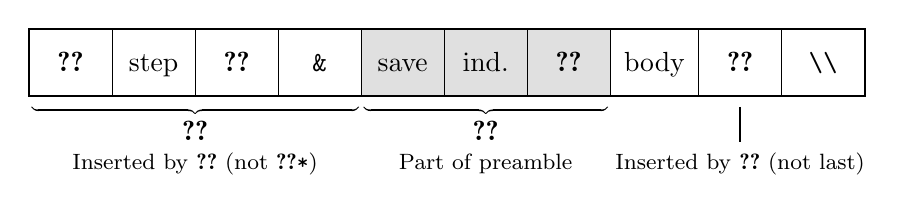
\begin{tikzpicture}
    \matrix (line) [
        matrix of nodes,
        % Hard-coding, or it would use semithick, rather than very thin:
        inner sep=-.1pt,
        row sep=-.2pt,
        column sep=-.2pt,
        nodes={
            inner xsep=.5em,
            inner ysep=2pt,
            rectangle,
            draw,
            very thin,
            minimum width=3em,
            minimum height=24pt,
            text depth=.5ex,
            text height=2ex,
            nodes in empty cells,
        },
        ]
    {

        \refk{bol}
        & step
        & \refk{label}
        & \verb|&|
        & |[auto]| save
        & |[auto]| ind.
        & |[auto]| \refk{font}
        & body
        & \refk{eol}
        & \verb|\\|
        \\
    };

    \draw[semithick, decorate, decoration={calligraphic brace,mirror}]
        ($(line-1-1.south west)+(1pt,-4pt)$)
        --
        node[inner sep=0, midway, below=5pt] (prefix) {\refk{prefix}}
        ($(line-1-4.south east)+(-1pt,-4pt)$)
        ;

    \draw[semithick, decorate, decoration={calligraphic brace,mirror}]
        ($(line-1-5.south west)+(1pt,-4pt)$)
        --
        node[inner sep=0, midway, below=5pt] (setup) {\refk{setup}}
        ($(line-1-7.south east)+(-1pt,-4pt)$)
        ;

    \draw[overlay] (prefix.south) node[font=\footnotesize, below] {\strut Inserted by
        \refc{\bslash} (not
        \code{\refc{\bslash}*})};
    \draw (setup.south) node[font=\footnotesize, below] {\strut Part of preamble};

    \draw[semithick] (line-1-9.south) + (0,-4pt)
    -- (line-1-9.south |- setup.south) node[font=\footnotesize, below]
        {\strut Inserted by \refc{\bslash} (not last)};

    \draw[semithick] (line.south west) rectangle (line.north east);
\end{tikzpicture}
\end{center}

\noindent
The components in the \refk{prefix} are populated by the \refc{\bslash}
command (or the beginning of the environment), the ones in the \refk{setup} by
the \refk{preamble}, and the actual body is supplied by the user, inside the
environment, terminated by the row separator \refc{\bslash} (which then goes
on to populate the next row, and so on). The \refk{eol} part is also inserted
by \refc{\bslash}, except if it's used after the last line (where it doesn't
really do anything).\footnote{Thus, \refk{eol} acts more as a line
\emph{separator} than a line \emph{terminator}.} The following describes the
default behavior, which can be modified substantially by setting the
appropriate options (e.g., \refk{prefix} and \refk{setup}).

\begin{description}[style=sameline, font=\normalfont]
    \item[\refk{bol}] This field is inserted by \refc{\bslash} (and
        \code{\cs{begin}\braces{\refe{pseudo}}}) at the beginning of the
        following line, using the \refc{pseudobol} command. Because it's a the
        very beginning of the tabular row, it may be used for things like
        \cs{rowcolor} when highlighting lines (as with the \refk{hl} key).
    \item[step] This refers to a call to \cs{stepcounter*} (where \refk{*} is
        an alias for \refk{pseudoline}), getting the counter ready for the
        label itself. Note that this does \emph{not} use \cs{refstepcounter},
        so at this point the counter has not been saved yet (and so you should
        not use \cs{label} to refer to it at this point).
    \item[\refk{label}]
        This is where the numbering label is inserted, using
        \refc{pseudolabel}; initially, this inserts
        \code{\cs{arabic}\refk{*}}.
    \item[\code{\&}] At the end of the prefix is the column separator, closing
        the label column and beginning the code line column.
    \item[save] Now that we're in the column where the user will normally
        insert text and code, we save \refk{pseudoline} so it may be used with
        \cs{label} and \cs{ref}, etc. This is done using
        \refc{pseudosavelabel}, which first \emph{decrements} the counter (to
        undo the increment before the label) and then calls
        \cs{refstepcounter}.
    \item[ind.] Inserts the appropriate amount of indentation (with an indent
        step length set by \refk{indent-length} or \refk{indent-text} and the
        indentation level set by \code{+}/\code{-} flags or
        \refk{indent-level}), using \refc{pseudoindent}.
    \item[\refk{font}] Inserts the base font, using \refc{pseudofont}.
    \item[body] This is where the manually written body of the code line
        appears.
    \item[\refk{eol}] Inserted by the terminating \refc{\bslash} (using
        \refc{pseudoeol}), unless we're at the end of the environment. Useful,
        e.g., for taking actions such as a
        \pkg[https://ctan.org/pkg/beamer]{beamer} \cs{pause} (cf.,
        \refk{pause}) between the lines.\footnote{If the same action must be
        taken after the last line, you can simply insert it there
        manually.}
    \item[\refc{\bslash}] The row/line separator. Ends one line (inserting
        \refk{eol}) and begins another (inserting \refk{prefix}). As in
        tabulars in general, this command is also permitted after the final
        line of the environment, but there it does no real work (i.e., it does
        not insert \refk{eol} and does not start a new line).
\end{description}

\subsection{Command and key reference}
\label{sec:cmdandkeyref}

In addition to descriptions of the various commands and options/keys (in
alphabetical order), you'll find definitions of a couple of counters here
(\refk{*} and \refk{pseudoline}).

% Not really a key, of course -- a counter
\begin{docKey}{*}{}{}
    This counter is a duplicate of \refk{pseudoline}, available inside
    \refe{pseudo}. It makes it possible to simplify calls such as
    \code{\cs{arabic}\braces{\refk{pseudoline}}} to starred forms such as
    \cs{arabic*}, like in \pkg[https://ctan.org/pkg/enumitem]{enumitem}. These
    short forms are available (and intended) for use in \refk{label} and
    \refk{ref}.
\end{docKey}

\begin{docCommand}{..}{}
    This is a shortcut that hijacks the normal \cs{.}\@ accent command, so
    that if it is called with \code{.}\@ as an argument, the result is
    \cs{dts}. In other words, the command \cs{..}\@ is really the call
    \code{\cs{.}\braces{.}}. For any other arguments, the original \cs{.}\@ is
    used, so while \code{\$1\cs{..}n\$} produces $1\..n$, \code{\cs{.}o} still
    yields~\.o.
\end{docCommand}

\begin{docCommand}{==}{}
    This is a shortcut that hijacks the normal \cs{=} accent command, so that
    if it is called with \code{=} as an argument, the result is \cs{eqs}. In
    other words, the command \cs{==} is really the call
    \code{\cs{=}\braces{=}}. For any other arguments, the original \cs{=} is
    used, so while \code{\$x\cs{==}y\$} produces $x\==y$, \code{\cs{=}o} still
    yields \=o.

    In some contexts, this may not work because \cs{=} has reverted to its
    original meaning (as is currently the case if you try to use it within a
    custom float, as in \cref{sec:floats}, or a standard one such as
    \code{figure}). In this case, you can restore the \pkg{pseudo} meaning
    (and the \refc{==} shortcut) by using \refc{pseudoeq}. In some cases, you
    may want to just use \refc{eqs} instead.
\end{docCommand}

\begin{docCommand}{\protect\bslash}{\,\colOpt{+}%
    \,\colOpt{-}%
    \,\colOpt{*}\,%
    \colOpt{<\meta{overlay specification}>}\,\oarg{line options}}

    \parindent1.5em
    \noindent
    This row separator is the workhorse of the \pkg{pseudo} package. Just as
    in a \code{tabular} environment, it signals the end of a line. It is
    optional after the list line, where it doesn't do any work.
%
    The command may be followed by a series of one or more plus (\code{+})
    signs, each of which will increment the indentation level before starting
    a new line; similarly, it may be followed by one or more minus (\code{-})
    signs, each of which will decrement the indentation level.
%
    Normally, the command will insert a \refk{prefix} at the beginning of the
    new line; if the star (\code{*}) flag is used, this prefix is not
    inserted.

    The optional overlay specifications refer to the \refk{hl} key, so
    \code{\refc{\bslash}<3>} is equivalent to \code{\refc{\bslash}[hl<3>]}.
    This applies to the following line, as do other options set explicitly as
    optional arguments. Note that options are set locally, \emph{before} the
    new line (and a new scope) is started, so unless they are handled
    specifically (in order to carry over), they will have no effect. Thus,
    even though all options are available here, not all make sense. (Consult
    individual option keys for intended use.)

    The pluses and minuses are conceptually part of the command name, and
    there should be no whitespace before the
    star (\code{*}).
    %
    You are, however, free to insert whitespace before the overlay
    specification and the line options. This means that you may, for example,
    place the overlay specification at the beginning of the following line in
    the source.
\end{docCommand}

\begin{docCommand}{arabic*}{}
    See \refk{*}.
\end{docCommand}

\begin{docKey}{begin-tabular}{\,=\,\meta{commands}}{no default}
    The actual command for beginning the \code{tabular} or \code{tabular}-like
    environment used by \refe{pseudo}. Normally not needed, as the
    \code{tabular} behavior may be modified by other keys, but could be used
    to use some other tabular environment, e.g., from packages such as
    \pkg[https://ctan.org/pkg/tabularx]{tabularx} or
    \pkg[https://ctan.org/pkg/longtable]{longtable}.
\end{docKey}

\begin{docKey}{bol}{\,=\,\meta{commands}}{\initiallyempty}
    Used to set \refc{pseudobol}, which is inserted at the beginning of each
    line. See also \refk{bol-append} and \refk{bol-prepend}.
\end{docKey}

\begin{docKey}{bol-append}{\,=\,\meta{commands}}{no default}
    Locally appends \meta{commands} to \refk{bol}.
\end{docKey}

\begin{docKey}{bol-prepend}{\,=\,\meta{commands}}{no default}
    Similar to \refk{bol-append}, except that \meta{commands} are added to
    the \emph{beginning} of \refk{bol}.
\end{docKey}

\begin{docCommand}{cn}{\marg{name}}

    Indicates a constant (such as \cn{true} or \cn{nil}). First wraps the
    argument in \cs{textnormal} and then uses \refc{cnfont}. See also
    \refc{DeclarePseudoConstant}.
    \fontutil{constants}
    \pseudoshortcutted{cn}

\end{docCommand}

\begin{docKey}{cnfont}{\,=\,\meta{command}}{\initialkeyvalue{\cs{textsc}}}
    \fontkey{cn}
\end{docKey}
\begin{docCommand}{cnfont}{}
    \fontcmd{cn}
\end{docCommand}

\begin{docKey}{compact}{\,=\,\meta{boolean}}{default \code{true}, initially
    \code{false}}

    \parindent1.5em
    \noindent
    The \refe{pseudo} environment emulates the built-in \LaTeX\ lists when it
    comes to spacing above and below, in normal text. If the environment is
    part of an ongoing paragraph, paragraphs will be inserted above and below,
    along with whitespace specified by \refk{topsep} (and \refk{parskip}). If
    the environment begins a paragraph of its own, additional whitespace is
    added, as specified by \refk{partopsep}. It is also possible to specify
    space to insert to the left of the environment, using \refk{left-margin}.

    However, these spacing commands don't work well inside \cs{mbox},
    \cs{fbox}, etc. To avoid getting into trouble, \pkg{pseudo} determines
    that the environment should be \emph{compact}, and drop this surrounding
    space, if we're in inner horizontal mode at the beginning of the
    environment.

\begin{texexp}
% In preamble:
% \usepackage{tikz}
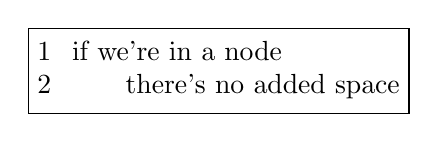
\begin{tikzpicture}
    \draw (0,0) node [draw] {%
        \begin{pseudo}
            if we're in a node \\+
                there's no added space
        \end{pseudo}};
\end{tikzpicture}
\end{texexp}

    This may not be enough, however. For example, if you're using
    \pkg[https://ctan.org/pkg/standalone]{standalone} to produce individual
    pseudocode images, this compactness may not be triggered automatically. In
    such cases, you can override the behavior using the \refk{compact} key,
    manually specifying whether you want the pseudocode to be compact or not.
\end{docKey}

\begin{docCommand}{ct}{\marg{text}}
    Indicates that \meta{text} is a comment, \ct{typeset like this}. You can
    customize the comment appearance using \refk{ctfont}, \refk{ct-left} and
    \refk{ct-right}:

\begin{texexp}
\pseudoset{
    ctfont=\color{black!75},
    ct-left=\unskip\qquad\texttt{/* },
    ct-right=\texttt{ */}
}
\begin{pseudo}
    $y=1$ \\
    $x=2$ \ct{this is a comment} \\
    $z=345$ \ct{this is another comment}
\end{pseudo}
\end{texexp}

    An alternative to using \refc{ct} is to simply set comments in a separate
    column, as demonstrated in \cref{sec:tabularx}. Or even without a separate
    column, if you use a \code{tabularx} as described there, and set the
    tabular width explicitly, you could insert an \cs{hfill} into
    \refk{ct-right} and get all end-markers aligned at the right-hand side:

    \medskip\noindent

    \begin{pseudo}[
        begin-tabular=\tabularx{\linewidth}{@{}r>{\pseudosetup}X@{}},
        end-tabular=\endtabularx,
        ctfont=\color{black!75},
        ct-left=\unskip\qquad\texttt{/* },
        ct-right=\hfill\texttt{ */}
        ]
        $x=1$ \\
        $y=2$  \ct{this is a comment} \\
        $z=345$ \ct{this is another comment}
    \end{pseudo}

    \medskip\noindent

    Or if you'd rather have the comments right-aligned (like you can in, e.g.,
    \pkg[https://ctan.org/pkg/algorithm2e]{algorithm2e}), you could use
    insert the \cs{hfill} at the beginning of the \refk{ct-left}:

    \medskip\noindent

    \begin{pseudo}[
        begin-tabular=\tabularx{\linewidth}{@{}r>{\pseudosetup}X@{}},
        end-tabular=\endtabularx,
        ctfont=\color{black!75},
        ct-left=\hfill\texttt{/* },
        ct-right=\texttt{ */}
        ]
        $x=1$ \\
        $y=2$  \ct{this is a comment} \\
        $z=345$ \ct{this is another comment}
    \end{pseudo}
\end{docCommand}

\begin{docKey}{ct-left}{\,=\,\meta{text}}{\initialkeyvalue{\code{(}}}
    \leftbracketing{comment}{ct}
\end{docKey}
\begin{docKey}{ct-right}{\,=\,\meta{text}}{\initialkeyvalue{\code{)}}}
    \rightbracketing{comment}{ct}
\end{docKey}
\begin{docKey}{ctfont}{}{\initialkeyvalue{\cs{textit}}}
    The font of the main text of a comment, when using \refc{ct}.
\end{docKey}
\begin{docCommand}{ctfont}{}
    \fontcmd{ct}
\end{docCommand}

\begin{docCommand}{DeclarePseudoComment}{\marg{shortcut}\marg{comment}}
    Used to declare a macro that expands to a comment. For example:
\begin{texexp}
\DeclarePseudoComment \Imp {Important!}
$x = y$ \qquad \Imp
\end{texexp}
    \seealsostyle{ct}
\end{docCommand}

\begin{docCommand}{DeclarePseudoConstant}{\marg{shortcut}\marg{constant}}
    Used to declare a macro that expands to a constant. For example:
\begin{texexp}
\DeclarePseudoConstant \False {false}
\False
\end{texexp}
    \seealsostyle{cn}
\end{docCommand}

\begin{docCommand}{DeclarePseudoFunction}{\marg{shortcut}\marg{function}}
    Used to declare a macro that expands to a function. For example:
\begin{texexp}
\DeclarePseudoFunction \Ln {length}
\Ln(A) or \Ln[A]
\end{texexp}
    \seealsostyle{fn}
\end{docCommand}

\begin{docCommand}{DeclarePseudoIdentifier}{\marg{shortcut}\marg{identifier}}
    Used to declare a macro that expands to a identifier. For example:
\begin{texexp}
\DeclarePseudoIdentifier \Rank {rank}
\Rank
\end{texexp}
    \seealsostyle{id}
\end{docCommand}

\begin{docCommand}{DeclarePseudoKeyword}{\marg{shortcut}\marg{keyword}}
    Used to declare a macro that expands to a keyword. For example:
\begin{texexp}
\DeclarePseudoKeyword \While {while}
\While
\end{texexp}
    \seealsostyle{kw}
\end{docCommand}

\begin{docCommand}{DeclarePseudoNormal}{\marg{shortcut}\marg{text}}
    Used to declare a macro that expands to normal text. For example:
\begin{texexp}
\DeclarePseudoNormal \Error {halt with an error message}
\begin{pseudo*}[kw]
    if $x \== \cn{nil}$ \\+
        \Error
\end{pseudo*}
\end{texexp}
    \seealsostyle{tn}
\end{docCommand}

\begin{docCommand}{DeclarePseudoProcedure}{\marg{shortcut}\marg{procedure}}
    Used to declare a macro that expands to a procedure. For example:
\begin{texexp}
\DeclarePseudoProcedure \Euclid {Euclid}
\Euclid(a, b)
\end{texexp}
    \seealsostyle{pr}
\end{docCommand}

\begin{docCommand}{DeclarePseudoString}{\marg{shortcut}\marg{string}}
    Used to declare a macro that expands to a string. For example:
\begin{texexp}
\DeclarePseudoString \Hello {Hello!}
\Hello
\end{texexp}
    \seealsostyle{st}
\end{docCommand}

\begin{docKey}{dim}{}{}
    Dims the following line. Equivalent to:
\begin{texexp}[listing only]
\pseudodefinestyle{dim}{
    bol-append   = \color{\pseudodimcolor},
    setup-append = \color{\pseudodimcolor}
}
\end{texexp}
May be used to dim out inactive or currently less relevant lines (possibly
using overlays; see~\cpageref{p:overlays}).
\begin{texexp}
\begin{pseudo}[kw, dim-color=black!25]*
\hd{Gnome-Sort}(A)                              \\
[dim]  $i = 1$                                  \\
[dim]  while $i \leq \fn{length}[A]$            \\+
           if $i \== 1$ or $A[i] \geq A[i-1]$   \\+
               $i = i + 1$                      \\-
[dim]      else \nf swap $A[i]$ and $A[i-1]$    \\+
[dim]          $i = i - 1$
\end{pseudo}
\end{texexp}
See also \refk{bol-append}, \refk{setup-append} and \refk{dim-color}.
\end{docKey}

\begin{docKey}{dim-color}{\,=\,\meta{color}}{no default, initially
    \cs{pseudohlcolor}}
    Sets the color used by \refk{dim} (available as \cs{pseudodimcolor}). The
    initial value is the one set by \refk{hl-color}.
\end{docKey}

% Wirth notation, Pascal
% https://proofwiki.org/wiki/Definition:Real_Interval/Notation/Wirth
% https://en.wikipedia.org/wiki/Ellipsis_(computer_programming)
\begin{docCommand}{dts}{} % The name in Concrete Mathematics
    A two-dot ellipsis, for use in the Wirth interval notation $1\..n$,
    typeset as \citeauthor{Graham:1994} did in
    \citetitle{Graham:1994}~\citep{Graham:1994}. Its definition is the same as
    in \pkg[https://ctan.org/pkg/gkpmac]{gkpmac}. Also accessible via the
    \refc{..} shortcut.
\end{docCommand}

\begin{docKey}{end-tabular}{}{\initialkeyvalue{\code{\cs{end}\braces{tabular}}}}
    The actual command for ending the \code{tabular} or \code{tabular}-like
    environment used by \refe{pseudo}. (See \refk{begin-tabular}.)
\end{docKey}

\begin{docKey}{eol}{\,=\,\meta{commands}}{\initiallyempty}
    Sets \refc{pseudoeol}, which is inserted at the end of all but the last
    line by \refc{\bslash}. See also \refk{eol-append} and \refk{eol-prepend}.
\end{docKey}

\begin{docKey}{eol-append}{\,=\,\meta{commands}}{no default}
    Locally appends \meta{commands} to \refk{eol}.
\end{docKey}

\begin{docKey}{eol-prepend}{\,=\,\meta{commands}}{no default}
    Similar to \refk{eol-append}, except that \meta{commands} are added to
    the \emph{beginning} of \refk{eol}.
\end{docKey}

\begin{docCommand}{eqs}{}
    Two equality signs typeset together as a binary relation, as in $x \eqs
    y$ (as opposed to the wider $x == y$, resulting from \code*{\$x == y\$}).
    It emulates the \pkg[https://ctan.org/pkg/stix]{stix} symbol \cs{eqeq},
    but for use with Computer Modern (the default \LaTeX\ font) or Latin
    Modern (available via the
    \pkg[https://ctan.org/tex-archive/info/lmodern]{lmodern} package). It
    should work just fine with other fonts. Also accessible via the \refc{==}
    shortcut, and configurable via \refk{eqs-pad}, \refk{eqs-scale} and
    \refk{eqs-sep}.
\end{docCommand}
\begin{docKey}{eqs-pad}{\,=\,\meta{muskip}}{\initialkeyvalue{\code{0.28mu}}}
    The amount of space inserted on each side of \refc{eqs}.
\end{docKey}
\begin{docKey}{eqs-scale}{\,=\,\meta{number}}{\initialkeyvalue{\code{0.6785}}}
    The amount of horizontal scaling applied to the \code{=} signs in
    \refc{eqs}.
\end{docKey}
\begin{docKey}{eqs-sep}{\,=\,\meta{muskip}}{\initialkeyvalue{\code{0.63mu}}}
    The amount of space inserted between the two \code{=} signs in \cs{eqs}.
\end{docKey}

\begin{docCommand}{fn}{\marg{name}\colOpt{(\meta{arguments})}}

    Indicates a function name, such as \fn{length}, and is initially
    more or less an alias for \refc{id}. The optional arguments (given in
    parentheses) are typeset in math mode, so
    \code{\cs{fn}\braces{length}(A)} yields \fn{length}(A).
    %
    Sometimes square brackets are used with functions that are meant to
    indicate array lookups or some property access or the like. This works in
    the same manner, so
    \code{\cs{fn}\braces{length}[A]} yields \fn{length}[A]. This behavior of
    picking up arguments carries over if you define a shortcut, of course:
\begin{texexp}
\def\Ln{\fn{length}}
We're not in math mode, but the argument of \Ln[A] is.
\end{texexp}

    % Should typeset \fn{test}[A] followed by (B) in normalfont:
    % \fn{test}[A](B)
    % Should typeset \fn{test}(A) followed by [B] in normalfont:
    % \fn{test}(A)[B]
    See also \refc{DeclarePseudoFunction}.
    \fontutil{function names}
    \pseudoshortcutted{fn}
\end{docCommand}

\begin{docKey}{fnfont}{\,=\,\meta{font}}{\initialkeyvalue{\refc{idfont}}}
    \fontkey{fn}
\end{docKey}
\begin{docCommand}{fnfont}{}
    \fontcmd{fn}
\end{docCommand}

\begin{docKey}{font}{\,=\,\meta{command}}%
    {\initialkeyvalue{\cs{normalfont}}}
    Sets the base font used in the code lines. Initially, this is just
    \cs{normalfont}, but the \refk{kw} switch is a convenient way to set it to
    the keyword font \refc{kwfont}. This is presumed to be a common case,
    under the assumption that most of the pseudocode will consist of either
    keywords or mathematics. If you'd rather explicitly mark up your keywords,
    leaving \refk{font} as it is, you could use \refc{kw} (or
    \refc{DeclarePseudoKeyword} for common cases):
\begin{texexp}
\begin{pseudo*}
\kw{while} pigs don't fly                       \\+
    keep waiting
\end{pseudo*}
\end{texexp}
\end{docKey}

\begin{docCommand}{hd}{\marg{name}(\meta{arguments})}
    Typesets a procedure signature, like \refc{pr}, but is intended for use as
    a \emph{header} for a procedure, rather than a procedure call. The
    difference is that \cs{hd} wraps its contents in a \cs{multicolumn},
    spanning two columns (i.e., both the label column and the main code
    column, but not any additional columns added using \refk{preamble} or
    \refk{begin-tabular}), using the preamble set with \refk{hd-preamble}. For
    this to work, you need to use the star flag (\code{*}) to suppress the
    automatic insertion of the \refk{prefix}:

\begin{texexp}
\begin{pseudo}*
    \hd{Algorithm}(x, y, z)                     \\
    setup                                       \\
    \kw{while} condition                        \\+
        iterative step                          \\-
    \kw{return} result
\end{pseudo}
\end{texexp}

    Note that the arguments are mandatory; in order to function properly,
    \cs{hd} must be \emph{expandable}, and therefore cannot end with an
    optional argument, the way \refc{pr} does.
    \pseudoshortcutted{hd}
\end{docCommand}

\begin{docKey}{hd-preamble}{\,=\,\meta{columns}}{no default}
    Sets the preamble used by \refc{hd}. The result is available as the column
    type with name \cs{pseudohdpreamble}. (Note that this is the literal
    column name, and not a macro containing the name. See \refk{preamble} for
    more information.) Initially, a single left-aligned column with
    \refc{pseudohpad} on either side (see \cpageref{p:hdpreamble}). If you
    introduce more columns in \refk{preamble}, you might want to increase the
    number of columns in \refk{hd-preamble} as well, or at least remove the
    right-hand \refc{pseudohpad}.
\end{docKey}

\begin{docKey}{hl}{}{\novaluekey}
    Prepends \refc{pseudohl} to \refk{bol}. Normally used with
    \pkg[https://ctan.org/pkg/beamer]{beamer} (see \cpageref{p:overlays}).
\end{docKey}

\begin{docKey}{hl-color}{\,=\,\meta{color}}{\initialkeyvalue{\code{black!12}}}
    Sets the color used by \refc{pseudohl} (available as \cs{pseudohlcolor}).
\end{docKey}

\begin{docKey}{hpad}{\,=\,\meta{length}}%
    {default \code{0.3em}, initially \code{0em}}
    Horizontal padding on either side of the pseudocode. Useful, among other
    things when highlighting lines, to have some of the highlighting (i.e.,
    row color) protrude beyond the text.
\end{docKey}

\begin{docKey}{hsep}{\,=\,\meta{length}}%
    {\initialkeyvalue{\code{0.75em}}}
    The space between the line labels and the code lines, i.e., between the
    two columns of numbered \refEnv*{pseudo} environments.
\end{docKey}

\begin{docCommand}{id}{\marg{name}}
    Indicates an identifier, and is simply an alias for \cs{textit} wrapped in
    \cs{textnormal}.
    See also \refc{DeclarePseudoIdentifier}.
    \fontutil{identifiers}
    \pseudoshortcutted{id}

    \medskip

    It might seem more natural to use \cs{mathit} (without \refCom*{tn}), but
    that may not give the desired results. First of all, special characters
    will not behave as if they're parts of a name:

\begin{texexp}
$\mathit{foo-bar:baz}$
\end{texexp}

    This may be remedied, e.g., by using the (internal) command
    \cs{newmcodes@} from \pkg[https://ctan.org/pkg/amsopn]{amsopn}, but the
    kerning, spacing and font application in the result still leaves something
    to be desired:

\makeatletter
\begin{texexp}
$\mathit{\newmcodes@ foo-bar:baz}$
\end{texexp}
\makeatother

    Compare this to a simple \cs{textit}:

\begin{texexp}
$\textit{foo-bar:baz}$
\end{texexp}

    The decision to use \cs{textit} means that you can't use, say, subscripts
    or the like as pars of an identifier, or mix in greek letters or other
    mathematical symbols. Though you can still easily typeset things like
    $\id{foo-$\alpha$}$, you'll have to mix in the math mode more
    explicitly (in this case, \verb|$\id{foo-$\alpha$}$|).
%
    \pseudoshortcutted{id}
\end{docCommand}
\begin{docKey}{idfont}{\,=\,\meta{font}}{\initialkeyvalue{\cs{textit}}}
    \fontkey{id}
\end{docKey}
\begin{docCommand}{idfont}{}{}
    \fontcmd{id}
\end{docCommand}

\begin{docKey}{indent-length}{\,=\,\meta{length}}{\initiallyempty}
    How large each indentation step is. If this key is not specified,
    \refk{indent-text} is used to calculate one the indent length instead.
\end{docKey}

\begin{docKey}{indent-level}{\,=\,\meta{length}}{no default, initially \code{0}}
    Sets the current indentation level. This is most usefully set on
    \refe{pseudo} environment, in concert with \refk{start}:\footnote{The
    \cs{strut} here is just to even out spacing above and below the text,
    which doesn't have fixed-height lines like the pseudocode.}
\begin{texexp}
\begin{pseudo}
    this is                                     \\+
    the first part
\end{pseudo}

\medskip \strut
This is some text interrupting the code.
\medskip

\begin{pseudo}[start=3, indent-level=1]
    this is the                                 \\-
    second part
\end{pseudo}
\end{texexp}
\end{docKey}

\begin{docKey}{indent-mark}{\,=\,\meta{mark}}{default vertical line, initially
    empty}
\def\algoexample#1{%
\begin{pseudo}[#1]
\kw{repeat} $n-1$ times \\+
    \kw{for} each edge $uv$ \\+
        update estimate for $v$ via $u$ \\--
\kw{for} each edge $uv$ \\+
    \kw{if} estimate for $v$ improves via $u$ \\+
        \kw{return} \cn{false} \\--
\kw{return} \cn{true}
\end{pseudo}
}

A mark used to indicate the start of each step of indentation. The
following example uses \verb|indent-mark=$\cdot$|:

\algoexample{indent-mark=$\cdot$}
%
By default, the indent mark is a vertical line with the same height and depth as
each row of the tabular used to typeset the pseudocode (i.e., it scales with
\refk{line-height}), so each indented block is indicated by a single unbroken
vertical line. The following example uses the \refk{indent-mark} key with no
argument:

\algoexample{indent-mark}
%
This default mark may be configured by using \refk{indent-mark-color} and
\refk{indent-mark-width}.
\end{docKey}

\begin{docKey}{indent-mark-color}{\,=\,\meta{color}}%
    {\initialkeyvalue{\codefont{lightgray}}}
    Sets the color to be used by the default \refk{indent-mark}.
\end{docKey}

\begin{docKey}{indent-mark-width}{\,=\,\meta{width}}%
    {\initialkeyvalue{\codefont{.6pt}}}
    Sets the width of the default \refk{indent-mark}.
    %
    The default value of \code{.6pt} corresponds to the
    \pkg[https://ctan.org/pkg/pgf]{tikz} line width \code{semithick}.
\end{docKey}

\begin{docKey}{indent-text}{\,=\,\meta{text}}%
    {\initialkeyvalue{%
    \code*{\cs{pseudofont}\cs{kw}\braces{else}\cs{\verbvisiblespace}}}}
    The size of each indentation step is set to the width of the \meta{text}.
    The default is set up so that code following on the same line as \kw{else}
    will be properly aligned, as in:

    \medskip

    \begin{pseudo*}[kw]
        if \tn{condition} \\+
            \tn{something} \\-
        else \tn{something else}
    \end{pseudo*}

    \medskip

    If you're not going to put code on the same line as \kw{else}, for
    example, you might want a different indentation size. To set it to some
    specific length, you could use
    the \refKey*{indent-length} key.
\end{docKey}

\begin{docKey}{kw}{}{\novaluekey}
    Sets \refk{font} to \refc{kwfont}.
\end{docKey}
\begin{docCommand}{kw}{\marg{name}}
    Indicates a keyword. First wraps the argument in \cs{textnormal} and then
    adds \cs{kwfont}.
    See also \refc{DeclarePseudoKeyword}.
    \fontutil{keywords}
    \pseudoshortcutted{kw}
\end{docCommand}

\begin{docKey}{kwfont}{\,=\,\meta{font}}{%
    \initialkeyvalue{\code{\cs{fontseries}\braces{b}\cs{selectfont}}}}
    \fontkey{kw}
    Note, however, that with the \refk{kw} switch, you set \code*{\refk{font}
    = \refc{kwfont}}, which is then applied as a font-switching command for
    each entire line, taking no argument. If you provide an command requiring
    an argument, the \refc{kw} command will still work, but the \refk{kw}
    switch won't:
\begin{texexp}
\pseudoset{kw}
\begin{pseudo*}[kwfont=\textsf]    % breaks kw option
    foo \kw{bar}
\end{pseudo*}
vs.\
\begin{pseudo*}[kwfont=\sffamily]  % works with kw option
    foo \kw{bar}
\end{pseudo*}
\end{texexp}
    The initial value isn't \emph{quite} as straightforward as indicated,
    however.
    For more info, see \refc{kwfont}.
\end{docKey}

\begin{docCommand}{kwfont}{}
    \parindent1.5em
    \noindent
    \fontcmd{kw}
    Its initial definition is \emph{essentially}
    \code{\cs{fontseries}\braces{b}\cs{selectfont}}, except the first time
    it's called (normally when evaluating the initial value of
    \refk{indent-text}), it also runs a check to see if the font selection
    \emph{worked}, as in some cases (such as in a default
    \pkg[https://ctan.org/pkg/beamer]{beamer} presentation), the non-extended
    bold may not be available. In that case, it defaults to an extended bold
    (\cs{bfseries}) instead. At this point, the command is redefined to
    \code{\cs{fontseries}\braces{b}\cs{selectfont}} or \cs{bfseries}, as
    appropriate (i.e., without this check). So, while
    \code{\refc{kw}\braces{hello}} produces the non-extended \kw{hello} in a
    default \LaTeX\ document, it yields the extended {\origbfseries\sffamily
    hello} in a default \pkg[https://ctan.org/pkg/beamer]{beamer}
    presentation. Perhaps more clearly, this is the result in plain \LaTeX\
    (using \pkg[https://ctan.org/tex-archive/info/lmodern]{lmodern}):

{\let\bfseries\origbfseries
\begin{texexp}
\textbf{while}\\                  % Extended
\kw{while}\\                      % Keyword
{\fontseries{b}\selectfont while} % Non-extended
\end{texexp}
}\ignorespaces\par

    \noindent
    The same code results in the the following in
    \pkg[https://ctan.org/pkg/beamer]{beamer}:

    \medskip\noindent
    \includegraphics{kwfig}

    \medskip\noindent
    You'll also get a font warning,\footnote{Of course, if you use a different
    font or theme, e.g., with the \pkg[https://ctan.org/pkg/beamer]{beamer}
    command \code{\cs{usefonttheme}\braces{serif}}, you may not have any issues to
    begin with.} though only once, as it's suppressed after the first occurrence,
    so the fact that the font selection doesn't work on the last line isn't
    reported. Note, however, that the current implementation of \refc{kwfont}
    actually \emph{piggybacks} on this warning to determine if the non-extended
    bold is available. This means that if you've tried (and failed) to use
    \code{\cs{fontseries}\braces{b}} \emph{before} the fist use of \refc{kwfont},
    the fallback (i.e., extended bold) won't be triggered.

    Also note that \refk{indent-text} (which will tend to be the first
    occurrence use of \refc{kwfont}) won't be evaluated (to determine
    \refk{indent-length}) until you actually start a \refe{pseudo}
    environment, so if you're \emph{aware} that you don't have non-extended
    bold available, and you set \code*{\refk{kwfont} = \cs{bfseries}}, for
    example, there will be no attempt to use the non-extended version, and you
    won't get the font warning that the default implementation produces in
    that case.
\end{docCommand}

\begin{docKey}{label}{\,=\,\meta{commands}}{%
    \initialkeyvalue{\code{\refc{arabic*}}}}%
\begin{texexp}
\pseudoset{kw, label=\footnotesize\arabic*:}

\begin{pseudo}
print \st{Hello, label!} \label{li:label} \\
goto \tn{\ref{li:label}}
\end{pseudo}
\end{texexp}

    Note that \cs{label} should be used in the actual code line, as here, and
    not in the number cell (which is generally not explicitly written,
    anyway).

    \medskip

    As kan be seen from the example, \cs{ref} is unaffected by
    \refKey*{label}, and in many cases that's what you want---as apposed to,
    say, ``\kw{goto} {\footnotesize 1:}''. In some cases, however (especially
    when using one of the other formatting commands, such as \cs{alph} or
    \cs{roman}), you \emph{do} want the reference format to reflect the
    original, or be similar in some way. To do that, you use the
    \refKey*{ref} key.
\end{docKey}

\begin{docKey}{label-align}{\,=\,\meta{column}}{\initialkeyvalue{\code{r}}}%
    Used to specify the alignment of the \refk{label} of each line. Whatever
    is provided is stored as a column type (named \cs{pseudolabelalign}),
    which is a part of the default \refk{preamble}. In other words, beyond the
    basic \code{l} and \code{r} (for left- and right-justified), you can
    supply anything that would be valid as part of the preamble (possibly
    using functionality from the \pkg[https://ctan.org/pkg/array]{array}
    package). If you want to get creative here, though, it might be easier to
    get the results you want by specifying your own \refk{preamble} in full.
\end{docKey}

\begin{docKey}{left-margin}{\,=\,\meta{length}}{\initialkeyvalue{\code{0pt}}}
    Sets the left margin of the \code{pseudo} environment, i.e., how far it is
    indented wrt.\ the surrounding text:
\begin{texexp}
Lorem ipsum dolor sit amet:

\begin{pseudo}[left-margin=1.25em]
consetetur sadipscing elitr \\
sed diam nonumy eirmod tempor
\end{pseudo}

Invidunt ut labore et dolore magna.
\end{texexp}

To have the environment indented as (the beginning of) any normal paragraph,
you could use \code*{left-margin = \cs{parindent}}. Note that
\refk{left-margin}, as well as the spacing above and below the \refe{pseudo}
environment, is turned off inside \cs{mbox} and the like:
\begin{texexp}
\pseudoset{left-margin=1cm} % Won't affect box contents
\fbox{\begin{pseudo*}
I'm a livin' in a box \\
I'm a livin' in a cardboard box
\end{pseudo*}}
\end{texexp}
Note that as opposed to \refk{topsep} and \refk{partopsep}, we are \emph{not}
working with one of the built-in list spacing commands; \cs{leftmargin} has no
effect on this key (which is why the hyphenated naming style of other keys such
as \refk{label-align} or \refk{indent-text} is also adopted for
\refk{left-margin}).
%
See also \refk{compact}.
\end{docKey}

\begin{docKey}{line-height}{\,=\,\meta{factor}}{\initialkeyvalue{\code{1}}}
    The \meta{factor} with which to multiply the ordinary line height. For
    simple, sparse pseudocode, the oridnary line height works well, but if
    your code
    gets too crowded with text and notation, you may wish to increase
    \code{line-height}. To emulate, e.g., the
    \cs{jot} set by
    \pkg[https://ctan.org/pkg/amsmath]{amsmath} (which is
    \code{0.25\cs{baselineskip}}), you could use \code{1.25}, though even
    \code{1.1} should help in many cases.
\end{docKey}

\begin{docCommand}{nf}{}
    Switch to the normal font (i.e., without bold or italics, etc.).
    \shortcutted{nf}{normalfont}
    See also \refc{tn}.
\end{docCommand}

\begin{docKey}{partopsep}{\,=\,\meta{length}}{\initialkeyvalue{\cs{partopsep}}}
    Sets a \pkg{pseudo}-local copy of \cs{partopsep} for use in vertical
    spacing above and below the \refe{pseudo} environment. See also \refk{compact}.
\end{docKey}

\begin{docKey}{pause}{}{\novaluekey}
    Equivalent to \code*{\refk{eol-append} = \cs{pause}} (see \cref{p:pause}).
\end{docKey}

\begin{docCommand}{pr}{\marg{name}\colOpt{(\meta{arguments})}}
    Indicates a procedure name, such as \cn{Quicksort}, and is initially
    more or less an alias for \refCom*{cn}. The optional arguments (in
    parentheses) are typeset in math mode, so
    \code{\cs{pr}\braces{Quicksort}(A,p,r)} yields \pr{Quicksort}(A,p,r).
    See also \refc{DeclarePseudoProcedure}.
    \fontutil{procedure names}
    \pseudoshortcutted{pr}
\end{docCommand}

\begin{docKey}{preamble}{\,=\,\meta{columns}}{no default}
    Sets the preamble to be used by the internal \code{tabular}. The result is
    available as the column type with name \cs{pseudopreamble}. (Note that
    this is the literal column name, and not a macro containing the name.
    Initially, \pkg{pseudo} uses a \code{tabular} as redefined by the
    \pkg[https://ctan.org/pkg/array]{array}, which prevents the expansion of
    whatever is provided as its preamble, and so we supply the preamble in the
    form of a single ``column'' instead.) For the default value, see the
    actual implementation on \cpageref{p:preamble} as well as the explanation
    in \cref{sec:linestructure}.
\end{docKey}

\begin{docKey}{prefix}{\,=\,\meta{commands}}{no default}
    This is the text inserted at the beginning of the following line by
    \refc{\bslash} (and by \code{\cs{begin}\braces{\refe{pseudo}}}), unless
    you use the star (\code{*}) flag. Unless modified, it inserts the code
    necessary to label the line and to move into the second column, where the
    actual code is inserted by the user. For the default value, see the actual
    implementation on \cpageref{p:prefix} as well as the explanation in
    \cref{sec:linestructure}.
\end{docKey}

\begin{docKey}{prfont}{\,=\,\meta{font}}{\initialkeyvalue{\refc{cnfont}}}
    \fontkey{pr}
\end{docKey}
\begin{docCommand}{prfont}{}
    \fontcmd{pr}
\end{docCommand}

\begin{docEnvironment}[doclang/environment content=pseudocode]%
    {pseudo}{\oarg{options}\,\colOpt{*}\,\colOpt{<\meta{overlay
    specification}>}\,\oarg{line options}}
    The actual environment in which the pseudocode is typeset. The
    \meta{options} are local to the environment, while the \meta{line options}
    are local to the following line (in the same manner as those set in
    \refc{\bslash}; i.e., only some will actually have any effect). The star
    (\code{*}) and \meta{overlay specification} act just like those on
    \refc{\bslash}. Note that if you wish to specify \meta{line options}
    without the star or the \meta{overlay specification}, you need to supply
    at least an empty pair of brackets for the global options:
\begin{texexp}
\begin{pseudo}[][hl]
First line \\
Second line
\end{pseudo}
vs.\
\begin{pseudo}[hl]
First line \\
Second line
\end{pseudo}
\end{texexp}
    There are no \code{+}/\code{-} flags here, unlike for \refc{\bslash};
    if needed, you can use \refk{indent-level}.
\end{docEnvironment}

\begin{docEnvironment}[doclang/environment content=pseudocode]%
    {pseudo*}{\oarg{options}\,\colOpt{*}\,\colOpt{<\meta{overlay
    specification}>}\,\oarg{line options}}
    An unnumbered version of the \refe{pseudo} environment. Equivalent to
    \refe{pseudo}, but with the \code{starred} style applied
    (see~\cpageref{p:starred}). Unless this style is altered, this means that
    the label column is removed from the preamble, and the prefix is reduced
    to only \refk{bol}.
\end{docEnvironment}

\begin{docCommand}{pseudobol}{}
    \setandused{bol}{pseudoprefix}
\end{docCommand}

\begin{docCommand}{pseudodefinestyle}{\marg{name}\marg{options}}
    Used to define ``styles'' or meta-keys, i.e., shortcuts for setting
    several keys to given values (used, e.g., to define \refk{starred}). The
    \meta{name} is simply the name of the new meta-key, and the \meta{options}
    are just what you'd provide to, e.g., \refc{pseudoset}.
\end{docCommand}

\begin{docCommand}{pseudoeol}{}
    \setandused{eol}{\bslash}
    It is inserted between lines, but not after the last one.
\end{docCommand}

\begin{docCommand}{pseudoeq}{}
    Similar to \refc{pseudoslash}. Switches the definition of \cs{=} to the
    one used by \pkg{pseudo}. Useful if \cs{=} reverts to its original
    definition in some context (see \refc{==}).
\end{docCommand}

\begin{docCommand}{pseudofont}{}
    \setandused{font}{pseudosetup}
    It is used to set up the font for each pseudocode line. (See also
    \refk{kw}.)
\end{docCommand}

\begin{docCommand}{pseudohl}{}
    This is the command inserted as \refk{bol} by the \refk{hl} switch.
    Initially, it's just a \cs{rowcolor} using the color set by
    \refk{hl-color}, but you could redefine it to whatever you wish.
\end{docCommand}

\begin{docCommand}{pseudohpad}{}
    Used on the left- and right-hand sides of \refk{preamble}.
    Conceptually, it inserts the horizontal space specified by \refk{hpad}. To
    play nice with \cs{rowcolor}, however, it is not used in a
    \code{@\braces{\dots}} column; rather, it's placed in
    \code{>\braces{\dots}} and \code{<\braces{\dots}} modifiers, and the
    actual space inserted has \cs{tabcolsep} subtracted.
\end{docCommand}

\begin{docCommand}{pseudoindent}{}
    % Protrudes into the margin:
    % \setandused{indent-length}{pseudosetup}
    % Manual:
    The command set by the \refk{indent-length} option. Used in
    \refc{pseudosetup}.
    More precisely, \refk{indent-length} is stored textually, and is converted
    to the length \cs{pseudoindentlength} when entering a \refe{pseudo}
    environment (so that units like \code{em} and \code{ex} adapt to the
    current font). The \cs{pseudoindent} command then inserts a horizontal
    space of length $\cs{pseudoindentlength}\times\textit{current indent
    level}$.
\end{docCommand}

\begin{docCommand}{pseudolabel}{}
    \setandused{label}{pseudoprefix}
\end{docCommand}

% Counter, not key
\begin{docKey}{pseudoline}{}{}
    Counter for pseudocode lines. See also \refk{*}.
\end{docKey}

\begin{docCommand}{pseudoprefix}{}
    \setandused{prefix}{\bslash}
\end{docCommand}

\begin{docCommand}{pseudosavelabel}{}
    Used as part of \refc{pseudosetup} to save the \refk{pseudoline} counter
    for use in \cs{label} and \cs{ref}. The \refk{pseudoline} counter is
    \emph{incremented} as part of the \refc{pseudolabel} command, but that's
    done using a plain \cs{stepcounter}, as any use of \cs{label} will
    presumably be placed in the pseudocode line (i.e., the next column). To
    save the value there, \cs{pseudosavelabel} first \emph{decrements} the
    counter, and then uses \cs{refstepcounter}.
\end{docCommand}

\begin{docCommand}{pseudoset}{\marg{options}}
    Used to set the configuration keys of the \pkg{pseudo} package (using
    \pkg[https://ctan.org/pkg/l3kernel]{l3keys} with
    \code{pseudo} as the module). These may also be set as
    % package options (in \cs{usepackage}) and as
    optional arguments to the \refEnv*{pseudo} and \refEnv*{pseudo*}
    environments. For example, if you'd like to switch to \cs{rm} as your base
    font, you could use \code*{\cs{pseudoset}\braces{font = \cs{rm}}}.
\end{docCommand}

\begin{docCommand}{pseudosetup}{}
    The command set by the \refk{setup} option. Used as part of the
    \refk{preamble}.

    \medskip

    \emph{Not to be confused with \refc{pseudoset}.}
\end{docCommand}

\begin{docCommand}{pseudoslash}{}
    Command similar to the \cs{arrayslash} of the
    \pkg[https://ctan.org/pkg/array]{array} package. Switches the definition
    of \cs{\bslash} to the one used by \pkg{pseudo}. Useful if you've used
    some code that modifies \cs{\bslash} for its own purposes (such as
    \cs{raggedleft} or the like).
\end{docCommand}

\begin{docKey}{ref}{\,=\,\meta{commands}}{initially empty, default
    \refc{pseudolabel}}
    Shortcut for setting the \cs{thepseudoline} command. If used without
    arguments, it will use the value supplied to \refKey*{label}.
\begin{texexp}
\pseudoset {
    label = (\textsc{\alph*}),
    ref   = \Alph*,
    hsep  = .5em
}

\begin{pseudo}
print \st{Hello, ref!} \label{li:ref} \\
goto \tn{\ref{li:ref}}
\end{pseudo}
\end{texexp}
\end{docKey}

\begin{docKey}{setup}{\,=\,\meta{commands}}{no default}
    The setup part of each pseudocode line: Save the line counter
    (using the \refc{pseudosavelabel} command), insert the proper indentation
    (with \refc{pseudoindent}) and switch to the correct font
    (\refc{pseudofont}).

    \medskip

    Rather than setting \refk{setup} directly, you may wish to add commands
    using \refk{setup-append} or \refk{setup-prepend}.
\end{docKey}

\begin{docKey}{setup-append}{\,=\,\meta{commands}}{no default}
    Locally appends \meta{commands} to \refk{setup}.
\end{docKey}

\begin{docKey}{setup-prepend}{\,=\,\meta{commands}}{no default}
    Similar to \refk{setup-append}, except that \meta{commands} are added to
    the \emph{beginning} of \refk{setup}.
\end{docKey}

\begin{docCommand}{st}{\marg{string}}
    Typesets \meta{string} with added quotes using \refc{stfont}. (The entire
    thing is wrapped in \cs{textnormal}.) For example, \code*{print
    \cs{st}\braces{42}} yields:
    \begin{pseudo*}
        print \st{42}
    \end{pseudo*}
    See also \refc{DeclarePseudoString}.
    \fontutil{strings}
    \pseudoshortcutted{st}
\end{docCommand}

\begin{docKey}{st-left}{\,=\,\meta{text}}{no default, initially \code{``}}
    \leftbracketing{string}{st}
\end{docKey}

\begin{docKey}{st-right}{\,=\,\meta{text}}{no default, initially \code{''}}
    \rightbracketing{string}{st}
\end{docKey}


\begin{docKey}{starred}{}{\novaluekey}
    The style (defined by \refc{pseudodefinestyle}) used by the \refe{pseudo*}
    environment. You may modify this (again using \refc{pseudodefinestyle}) if
    you wish.
\end{docKey}

\begin{docKey}{start}{\,=\,\meta{number}}{no default, initially \code{1}}
    Sets the starting line number:
\begin{texexp}
\begin{pseudo}[start=10]
Maybe we're continuing from some earlier code?  \\
Anyway, let's keep going!
\end{pseudo}
\end{texexp}
See also \refk{indent-level}.
\end{docKey}

\begin{docKey}{stfont}{}{}
    \fontkey{st}
\end{docKey}

\begin{docCommand}{stfont}{}
    \fontcmd{st}
\end{docCommand}

\begin{docCommand}{tn}{\marg{text}}
    An alias for \cs{textnormal}, to break out of the font set using the
    \refKey*{font} key, for inserting ordinary prose between the keywords. For
    example, to get the result ``{\kwfont for \tn{every node} $v\in V$}'', one
    might write:

    \medskip

    \centerline{\code{for \cs{tn}\braces{every node} \$v\cs{in} V\$}}

    \medskip

    This is equivalent to using \code*{\cs{textnormal}\braces{every node}}.
    \shortcutted{tn}{textnormal}
\end{docCommand}

\begin{docKey}{topsep}{\,=\,\meta{length}}{\initialkeyvalue{\cs{topsep}}}
    Sets a \pkg{pseudo}-local copy of \cs{topsep} for use in vertical spacing
    above and below the \refe{pseudo} environment. See also \refk{compact}.
\end{docKey}

\begin{docKey}{unknown}{}{}
    Unknown keys are checked for \pkg[https://ctan.org/pkg/beamer]{beamer}
    overlay specifications. That is, if an unknown key has the form

    \medskip

    \centerline{\code*{\meta{name}<\meta{overlay
    specification}> = \meta{value}}}

    \medskip

    then it does not trigger an error, but, if
    \pkg[https://ctan.org/pkg/beamer]{beamer} is used, is rewritten to:

    \medskip

    \centerline{\code*{\cs{only}<\meta{overlay specification}>\braces{%
        \refc{pseudoset}\braces{\meta{name} = \meta{value}}%
    }}}

    \medskip

    If \pkg[https://ctan.org/pkg/beamer]{beamer} is \emph{not} used, the key
    is simply ignored. Note that because of current limitations on how keys
    are handled,
    % Cf. https://github.com/latex3/latex3/issues/67
    unknown keys cannot have defaults, and so there is no way to insert a
    marker for when no value is provided, which could be used to determine
    whether to use
    \code*{\refc{pseudoset}\braces{\meta{name} = \meta{value}}}
    or simply
    \code*{\refc{pseudoset}\braces{\meta{name}}}. Instead, if an empty value
    is provided to the unknown key, that is treated in the same way as when
    the key is used
    without a value, resulting in
    \code*{\refc{pseudoset}\braces{\meta{name}}}
    rather than
    \code*{\refc{pseudoset}\braces{\meta{name} = }}.
\end{docKey}

\section{But how do I\,\dots}

Some functionality is not built in, but is still fairly easy to achieve. Some
streamlining may be added in future versions.

\subsection{\dots\,prevent paragraph indentation after \code{pseudo}?}

If you want to keep the pseudocode as part of a surrounding paragraph, you
could have it not start its own, i.e., not have an empty line before it. This
will reduce the amount of spacing as well; if you'd rather have that reduced,
you could simply drop the empty line \emph{after} the environment:

\begin{texexp}[listing only]
Text before

\begin{pseudo}
    pseudocode
\end{pseudo}
%
Text after
\end{texexp}

\noindent
The effect would then be the following:

\begin{pseudo}
    pseudocode
\end{pseudo}
%
No indentation here, and normal spacing. If, however, you wish to suppress
indentation after \emph{all} instances of \refe{pseudo}, you could use the
\pkg[https://ctan.org/pkg/noindentafter]{noindentafter} package, as follows:

\medskip

\begin{texexp}[listing only]
\usepackage{noindentafter}
\NoIndentAfterEnv{pseudo}
\end{texexp}

\noindent
If you wish to override this, and indent a given paragraph after all, you can
simply use the \cs{indent} command.

\subsection{\dots\,get log-like functions?}

There's no built-in command for math-roman function names, as used in $\log$
and $\sin$, etc. (other than just setting \refk{fnfont}, if you want it
everywhere). If you wish to define your own, you could use \cs{operatorname}
or \cs{DeclareMathOperator}. For example:

\begin{texexp}
% In preamble:
% \usepackage{amsmath}
% \DeclareMathOperator{\MyFunc}{my-func}
\begin{pseudo}[kw]
if $\MyFunc x \== 1$ \\+
    $y = \MyFunc(z + 1)$
\end{pseudo}
\end{texexp}

\noindent
The spacing is then correct whether you enclose the arguments in parentheses
or not.

\subsection{\dots\,unbold punctuation?}

If you use the \refk{kw} key, all pseudocode not in math mode will end up
using the keyword font (\refc{kwfont}), which initially is bold. Though some
\emph{do} typeset, e.g., grouping braces in boldface, you might not want to do
that; the same goes for, say, line-terminating semicolons. The
\code{theoremfont} option of, e.g., \pkg[https://ctan.org/pkg/newtx]{newtx}
does something similar (for italics), but uses a custom font for that.
Packages like \pkg[https://ctan.org/pkg/embrac]{emrac} rely on straightforward
textual substitution, replacing certain characters with marked-up ones, but
the way things are set up at the moment, our font command won't have access to
the entire line when it's executed.

If you're adventurous, it's not hard (using the
\pkg[https://ctan.org/pkg/xparse]{xparse} argument type \code{u}) to make a
version that \emph{does} gobble up the entire line, up to and including
\verb|\\| (and you could then use the regular expression functionality from
\pkg[https://ctan.org/pkg/expl3]{expl3}, presumably also reinserting
\refc{\bslash}). A simpler solution is to just use \refc{DeclarePseudoNormal}.
Here's an example based on pseudocode from \citet{Knuth:1975}:

\begin{texexp}
% \usepackage{mathtools}
\let\gets\coloneqq

\pseudoset{kw, indent-length=2em, line-height=1.1}

\DeclarePseudoNormal \; ;

\begin{pseudo*}
procedure \id{printstatistics}\;                            \\
begin integer $j$\;                                         \\+
    $\id{write}(\st{Closed sets for rank}, r, \st{:})$\;    \\
    $j \gets L[h]$\;                                        \\
    while $j \neq h$ do                                     \\+
        begin $\id{writeon}(S[j])$\; $j\gets L[j]$ end\;    \\--
end\;
\end{pseudo*}
\end{texexp}

\noindent
If you'd really like to avoid the extra backslashes, you could make the
relevant punctuation active (though that's probably a bit risky; make sure to
only do it locally, at the very least):

\begin{texexp}
\DeclarePseudoNormal \semi ;

\catcode`\;=\active
\let;\semi

\begin{pseudo*}[kw]
    begin integer $j$; % Look! The semicolon isn't bold!
\end{pseudo*}
\end{texexp}

\subsection{\dots\,use \texttt{tabularx}?}
\label{sec:tabularx}

You can use other tabular packages such as
\pkg[https://ctan.org/pkg/tabularx]{tabularx} via \refk{begin-tabular} and
\refk{end-tabular}. Let's say, for example, that you wish to extend the
\refe{pseudo} environment to fill out the entire line, and set up a new column
for comments. You could achieve that as follows:

% ! Duplicate of the one inside texexp, so it can be reused later.
\pseudodefinestyle{fullwidth}{
    begin-tabular =
    \tabularx{\linewidth}{@{}
        r                                      % Labels
        >{\pseudosetup}                        % Indent, font, ...
        X                                      % Code (flexible)
        >{\leavevmode\small\color{black!60}}   % Comment styling
        p{0.45\linewidth}                      % Comments (fixed)
        @{}},
    end-tabular=\endtabularx
}
\begin{texexp}
\pseudodefinestyle{fullwidth}{
    begin-tabular =
    \tabularx{\linewidth}{@{}
        r                                      % Labels
        >{\pseudosetup}                        % Indent, font, ...
        X                                      % Code (flexible)
        >{\leavevmode\small\color{black!60}}   % Comment styling
        p{0.45\linewidth}                      % Comments (fixed)
        @{}},
    end-tabular = \endtabularx,
    setup-append = \pseudoeq
}
\begin{pseudo}[kw, fullwidth, line-height=1.1]*
    \hd{Counting-Sort}(A, k) & Find positions by counting \\
    $C = \tn{an array of $k$ zeros}$ & Element frequencies \\
    for $i = 1$ to $A.\id{length}$ & Count all elements \\+
    $\dots$ & Etc.
\end{pseudo}
\end{texexp}
%
Note that using the \cs{color} command in a \code{>\braces{\dots}}
modifier with a \code{p} column places the text in a new paragraph, on the
next line; you'll need to insert \cs{leavevmode} or the like to prevent that.
This is true also of normal \code{tabular} environments. Also note
that \code{tabularx} environments with \code{X} columns don't interact nicely
with \cs{=}; so if you wish to use \refc{==}, you can reassert the definition
by adding \code{>\braces{\refc{pseudoeq}}} before each column.

See the \pkg[https://ctan.org/pkg/tabularx]{tabularx} documentation
(page~4) for an explanation of why we can't use
\code{\cs{begin}\braces{tabularx}} and \code{\cs{end}\braces{tabularx}}.
Also note that because \pkg[https://ctan.org/pkg/tabularx]{tabularx} passes
its contents as the argument to a macro, the parsing \pkg{pseudo} uses to
determine if \refc{\bslash} is at the end of the last line doesn't work; if
you add \refc{\bslash} at the end here, you'll introduce an empty line.

\makeatletter
For simplicity, I've used \code{@\braces{}} to remove space on either side.
For \refk{hpad} to work, you should use \code{>\braces{\cs{pseudohpad}}} and
\code{<\braces{\cs{pseudohpad}}} instead, as in the standard \refk{preamble}
(see \cpageref{p:preamble}). To keep things configurable, you might also want
to use \cs{pseudolabelalign}, rather than \code{r}.
\makeatother

\subsection{\dots\,get tab stops?}

Some packages, such as \pkg[https://ctan.org/pkg/clrscode3e]{clrscode3e}, use
an actual \code{tabbing} environment internally. While this may be a bit
brittle (e.g., creating problems if you wish to insert your pseudocode into a
\pkg[https://ctan.org/pkg/pgf]{tikz} node---one of the goals of \pkg{pseudo}),
it does mean that you can use the tabbing command \cs{>} manually, to align
various construct.

If all your tabbing is done \emph{before} the text on a given code line, you
can achieve this in \pkg{pseudo} as well, by using the \code{+} and \code{-}
modifiers. (For example, the tab stops in
\pkg[https://ctan.org/pkg/clrscode3e]{clrscode3e} are set at fixed intervals,
just like in \pkg{pseudo}.) But what if you'd like to align something that
comes later, such as comments after code lines? You can't simply use
\cs{hspace}, of course, unless the code lines themselves have exactly the same
length.

One solution is to use an additional column, as discussed in
\cref{sec:tabularx}, but you could also make creative use of the \cs{rlap}
command, which prevents its contents from taking up horizontal space:%
\footnote{Note that \cs{rlap} doesn't start a new paragraph, which is why I
use \cs{noindent}, here. You could replace
\code{\cs{noindent}\cs{rlap}\braces{\dots}} with
\code{\cs{makebox}[0pt][l]\braces{\dots}}. This isn't an issue in
\code{pseudo} code lines, however.}


\begin{texexp}
\noindent\rlap{This is some text}%
And here is some more
\end{texexp}

\noindent
By using \cs{rlap} on the code lines in question, you can insert \cs{hspace}
that begins at the beginning of the code line (here with an example
convenience command defined using \pkg[https://ctan.org/pkg/xparse]{xparse}):

\begin{texexp}
\NewDocumentCommand \C { +u{/* } +u{ */} } {%
    \rlap{#1}\hspace{3cm}\ct{#2}\\%
}
\begin{pseudo}
\C $x = 42$      /* first comment */
\C $y = \sin x$  /* second comment */
\end{pseudo}
\end{texexp}

\noindent
See also the discussion of the \refc{ct} command for ideas on typesetting
comments. If you wish to align things across different indentation levels,
you'll have to add or subtract multiples of \cs{pseudoindentlength} (see
\refc{pseudoindent}).

\subsection{\dots\,use horizontal lines?}
\label{sec:horizontallines}

Many opt for a table-like appearance when typesetting algorithms, with
horizontal lines above and below, and generally a header row on top. While
this may be part of a surrounding floating environment (see
\cref{sec:floats}), you may also wish to include such lines in your actual
pseudocode. In this case, you can simply use existing \code{tabular}-based
tools such as \pkg[https://ctan.org/pkg/booktabs]{booktabs}, making sure to
suppress the \pkg{pseudo} \refk{prefix} using the star flag (\code{*}):

\begin{texexp}
% \usepackage{booktabs}
\begin{pseudo}*
\toprule

    \hd{Bor\r{u}vka}(G, w)                      \\
                                                %
[bol=\midrule]

    \kw{while} $E(G)$ is not empty              \\+
        \kw{for} each $u\in V(G)$               \\+
            add light $uv \in E(G)$ to $T$      \\-
        \kw{for} each $e \in T$                 \\+
            contract $e$                        \\*

\bottomrule
\end{pseudo}
\end{texexp}

\noindent
Rather than \code{\cs{\bslash}[bol=\cs{midrule}]}, you could also have used
\code{\cs{\bslash}*}, followed by \code{\cs{midrule}\cs{pseudoprefix}}. (Note
that the paragraph break between \refc{\bslash} and its argument has been
commented out.)

\subsection{\dots\,get an algorithm float?}
\label{sec:floats}

There are (at least) two different ways of viewing a block of pseudocode: As
an inline element, like equations, or as a float, like figures and tables. For
example, \citet{Cormen:2009} place their pseudocode inline, and refer to the
algorithms by name (e.g., \pr{Dijkstra}), while \citet{Williamson:2011} place
them in floats, and refer to them by number (e.g.,
Algorithm~3.1).%
\footnote{A third option that is sometimes used is to use a theorem-like
environment for your algorithms. There are many packages to help with this;
just search \href{https://ctan.org}{\textsc{ctan}} for
``\href{https://ctan.org/search/?phrase=theorem}{theorem}''.}
%
Some pseudocode packages have a custom float environment (à la \code{table}
and \code{figure}) for use with algorithms described by pseudocode. Beyond
having a new float name (such as ``Algorithm'') with its own numbering and the
like, they at times have rather distinct styling (horizontal lines in
\pkg[https://ctan.org/pkg/algorithms]{algorithms} and
\pkg[https://ctan.org/pkg/algorithmicx]{algorithmicx}, and a surrounding box
in \pkg[https://ctan.org/pkg/algorithm2e]{algorithm2e}), which may or may not
suit the styling of the rest of your document.

Rather than getting into the business of float environments, I leave such
things to separate packages designed for that use. A basic solution would be
to simply use the \pkg[https://ctan.org/pkg/float]{float} package (which also
provides ruled and boxed floats, should you wish to have those), but a quick
\href{https://ctan.org}{\textsc{ctan}} search for
``\href{https://ctan.org/search/?phrase=float}{float}'', or a look at the
\href{https://ctan.org/recommendations/float}{recommendations} related to the
\pkg[https://ctan.org/pkg/float]{float} package, will give you many options,
with varying functionality.
%

\medskip

\paragraph{Note:} The definition of \refc{==} doesn't properly carry over into
floats. It's properly redefined inside \refe{pseudo}, so you probably won't
notice, but if you wish to use the symbol outside the \refe{pseudo}
environment, but in a float (e.g., inside \cs{caption}), you'll need to either
call \refc{pseudoeq} to re-establish the definition of \cs{=} or simply use
\refc{eqs} instead of \refc{==}.

\medskip

\noindent
Here's a simple example using the \pkg[https://ctan.org/pkg/float]{float}
and \pkg[https://ctan.org/pkg/caption]{caption} packages, reusing the
\code{fullwidth} style example from \cref{sec:tabularx} and the horizontal
line ideas from \cref{sec:horizontallines}:

% ! Duplicate of the code in the actual float
\begin{texexp}[listing only]
% \usepackage{float}
% \usepackage{caption}
\floatstyle{plaintop}
\newfloat{algorithm}{tbp}{alg}[section]
\floatname{algorithm}{Algorithm}

\begin{algorithm}
\begin{pseudo}[fullwidth]*

% Insert pseudocode and comments

\end{pseudo}
\caption{...}
\end{algorithm}
\end{texexp}

\noindent
You can see the result in \cref{alg:example}.

\floatstyle{plaintop}
\newfloat{algorithm}{tbp}{alg}[section]
\floatname{algorithm}{Algorithm}
\begin{algorithm}
\begin{pseudo}[fullwidth]*
\toprule

    \hd{Bor\r{u}vka}(G, w) &
        Construct MST $T$ for $G$ wrt.\ $w$ \\[bol=\midrule]

    \kw{while} $E(G)$ is not empty &
        Not all are contracted yet \\+
        \kw{for} each $u\in V(G)$ &
            One light edge per node \\+
            add light $uv \in E(G)$ to $T$ &
            $T$ is the tree we're building \\-
        \kw{for} each $e \in T$ &
            These edges are already used \\+
            contract $e$ &
            We focus on the remaining ones \\*

\bottomrule
\end{pseudo}
\caption{Bor\r{u}vka's algorithm for finding minimum spanning trees. For a
node $u$, a \emph{light} edge is an edge $uv$ of minimum weight $w(u,v)$.
Contracting $uv$ deletes it, identifies $u$ and $v$, and removes resulting
loops. The result $T$ is initially empty.}
\label{alg:example}
\end{algorithm}

\subsection{\dots\,handle object attributes?}

In the \pkg[https://ctan.org/pkg/clrscode3e]{clrscode3e} package, you'll find
an assortment of commands for handling
object attributes such as $A.\id{length}$. The manual says (here with emulated
kerning of the dot operator):

\begin{quote}
    You might think you could typeset $A\mkern1mu.\id{length}$ by
    \code{\$A.\cs{id}\braces{length}\$}, but that would produce
    $A\mkern1mu.\mkern-1.5mu\id{length}$, which has not quite enough space
    after the dot. \hfill(page~3)
\end{quote}

\noindent
However, this is a font issue, more than anything. If, for example, if you
want Times New Roman (like Cormen et al.)\@ and use
\pkg[https://ctan.org/pkg/mathptm]{mathptm}, you at times run into the problem
described; with \pkg[https://ctan.org/pkg/newtx]{newtx} it's less pronounced.
With other fonts (e.g.,
\pkg[https://ctan.org/pkg/fourier]{fourier},
\pkg[https://ctan.org/pkg/mathpple]{mathpple} or
\pkg[https://ctan.org/pkg/newtx]{newtxmath} with
\pkg[https://ctan.org/pkg/libertine]{libertine}), or even without any font
packages (or possibly using \pkg{lmodern}), the kerning works just fine.

In general, then, I suggest you try to use \code{\$A.\cs{id}\braces{length}\$}
and the like, and see if the result is satisfactory:

\begin{texexp}
$v.\id{prev}.\id{next} = v.\id{next}$
\end{texexp}

\noindent
If you \emph{do} need to adjust the kerning (with \cs{mkern} commands or
perhaps using \pkg[https://ctan.org/pkg/microtype]{microtype}), you may of
course do so, but \pkg{pseudo} does not (at present) include any special
attribute lookup commands that do it for you.

\subsection{\dots\,indicate blocks with braces or the like?}

Some packages (such as \pkg{algorithm2e}) have support for using vertical lines
to indicate the block structure;
\pkg[https://ctan.org/tex-archive/macros/latex/contrib/pseudocode]{pseudocode}
uses large braces. In \pkg{pseudo}, there is support for using an
\refk{indent-mark}, for which the default is a semithick, gray vertical line
(see \cpageref{p:indent-mark}). However, by using
\pkg[https://ctan.org/pkg/pgf]{tikz}, you could draw all kinds of indentation
decorations.

You could, for example, add a \code{node} at the start of each code line,
containing an \verb|\@arstrut|, the (\pkg{array}) strut used to indicate the
extent of a tabular row:

% ! Contents duplicated
\makeatletter
\NewDocumentCommand \pseudoanchor { m } {%
    \tikz[baseline, overlay, remember picture]
        \node[anchor=base, inner sep=0] (#1) {\@arstrut};%
    \ignorespaces
}
\makeatother
\begin{texexp}[listing only]
% \usepackage{xparse,tikz}
% \usetikzlibrary{decorations.pathreplacing,calligraphy}
\makeatletter
\NewDocumentCommand \pseudoanchor { m } {%
    \tikz[baseline, overlay, remember picture]
        \node[anchor=base, inner sep=0] (#1) {\@arstrut};%
    \ignorespaces
}
\makeatother
\end{texexp}

\noindent
We can then use the resulting nodes to draw braces or lines or whatever. First
some example setup:

% ! Duplicated
\begin{texexp}[listing only]
\pseudoset{
    kw,
    indent-length = 3.5em,
    setup-append = {\pseudoanchor{L-\arabic*}}
}
\tikzset{
    braces/.style =
    {thick, decoration = {calligraphic brace, raise=.2em}},
    label/.style =
    {midway, left=3em, anchor=west, font=\strut\kwfont}
}
\end{texexp}
You would then get something like the following:
{
\pseudoset{
    kw,
    indent-length = 3.5em,
    setup-append = {\pseudoanchor{L-\arabic*}}
}
\tikzset{
    braces/.style =
    {thick, decoration = {calligraphic brace, raise=.2em}},
    label/.style =
    {midway, left=3em, anchor=west, font=\strut\kwfont}
}
\begin{texexp}
\begin{pseudo}
if $x < y$                                      \\+
    $x = y$                                     \\
    $y = 0$
\end{pseudo}
\tikz[overlay, remember picture, braces] {
    \draw[decorate] (L-3.south) -- (L-2.north) node[label] {then};
}
\end{texexp}
}

\noindent
If multiple blocks are closed at the same time, the bottom coordinates could be
things like \code*{(L-2.north |- L-3.south)} instead. To adjust the end
points, you could also use things like \code{(\$(L-3.south)+(0,.2em)\$)}.

The actual drawing of the brace (or line or whatever) isn't automated here, of
course. This could be done by some hook triggered by the \code{-} flags in
\refc{\bslash}. If it turns out there's a demand for something like that, I
might add it in a future version.

\subsection{\dots\,use \pkg{pseudo} with older \TeX\ distributions?}
\label{sec:older}

As mentioned in the introduction, I've tried to make \pkg{pseudo} work with at
least \emph{somewhat} outdated \TeX\ distributions. In these cases, the
package itself won't be available as part of the distribution, of course, but
you can simply download the file
\texttt{\href{http://mirrors.ctan.org/macros/latex/contrib/pseudo/pseudo.sty}{pseudo.sty}}
and place it in the directory where you're compiling your document (or
anywhere else where your \LaTeX\ executable can find it).

However, there may be cases where this just doesn't work, such as when
submitting to a publisher with a really old setup.\footnote{If possible,
though, feel free to
\href{https://github.com/mlhetland/pseudo.sty/issues}{file an issue} or
\href{https://github.com/mlhetland/pseudo.sty/pulls}{provide a pull request}
to address the issue.}
In that case, the simplest solution is probably to use the
\pkg[https://ctan.org/pkg/standalone]{standalone} package to produce
individual PDFs of your algorithms, and then to include those in your
document. Then you can submit the PDFs rather than the \LaTeX, so that the
pseudocode need not be compiled on the old system. Each algorithm could go in
a file like this:

\begin{texexp}[listing only]
\documentclass{standalone}
\usepackage{pseudo}
\begin{document}
\begin{pseudo}
    ...
\end{pseudo}
\end{document}
\end{texexp}

\noindent
Let's say this is compiled to \texttt{algo1.pdf}. You then include this file:

\begin{texexp}[listing only]
\documentclass{article}
\usepackage{graphicx} % For \includegraphics
...
\begin{document}
... sanctus est Lorem ipsum dolor sit amet:

\medskip\noindent
\includegraphics{algo1}

\smallskip
Lorem ipsum dolor sit amet, consetetur sadipscing ...
\end{document}
\end{texexp}

\noindent
Of course, you can adjust the spacing (e.g., using \verb|\vspace| or the like)
to your liking. Using this method, you can can achieve results essentially
identical to if you compiled the pseudocode directly as part of the document.
Of course, you won't have access to other functionality (such as
\verb|\DeclarePseudoIdentifier| or the like) for use in the main tex, but most
of that should be possible to emulate by hand (possibly peeking at the
implementation in \cref{sec:impl}).

\subsection{\dots\,use a header with no arguments?}

Normally, \refc{hd} has a mandatory set of arguments; at the very least,
you'll need to supply the parentheses:

\begin{texexp}
\begin{pseudo}*
\hd{No-Arguments}() \\
\dots\ but still with parentheses
\end{pseudo}
\end{texexp}

\noindent
This is because \refc{hd} has to be fully expandable to be able to insert the
requisite \cs{multicolumn}, and then it cannot have any (final) optional
arguments. If you'd like, though, you can just use \cs{multicolumn} yourself
(see also \refk{hd-preamble}):

\begin{texexp}
\begin{pseudo}*
\multicolumn{2}{\pseudohdpreamble}
{\pr{No-Arguments}} \\
\dots\ and no parentheses!
\end{pseudo}
\end{texexp}

\section{Implementation}
\label{sec:impl}

\lstdefinestyle{tcblatex}{language={[LaTeX]TeX},
    aboveskip={0\p@ \@plus 6\p@},
    belowskip={0\p@ \@plus 6\p@},
    columns=fullflexible,
    keepspaces=true,
    breaklines=true,
    breakatwhitespace=true,
    basicstyle=\ttfamily\small\color{black!80},
    keywordstyle=,
    extendedchars=true,
    nolol,
    inputencoding=\kvtcb@listingencoding,
    literate={VERSION}{\pseudoversion}{3}{DATE}{\pseudodate}{10},
}

\noindent
\textbf{Note:} In the following, \verb|_@@| and \verb|@@| represent
an internal prefix (\verb|__pseudo|), the same way they do with
\pkg[https://ctan.org/pkg/l3docstrip]{l3docstrip}.

\bigskip\noindent
First, we just define some metadata:
\begin{source}
\def \pseudoversion {VERSION}
\def \pseudodate    {DATE}
\end{source}
The \pkg{pseudo} package is implemented using experimental \LaTeX\,3, so we
start by importing \pkg[https://ctan.org/pkg/expl3]{expl3}:
\begin{source}
\RequirePackage{expl3}
\end{source}
Then we're ready start the package:
\begin{source}
\ProvidesExplPackage
    {pseudo}
    {\pseudodate}
    {\pseudoversion}
    {Straightforward pseudocode}
\end{source}
Tools for defining user commands:
\begin{source}
\RequirePackage{xparse}
\end{source}
The \refe{pseudo} environment is built upon tabular functionality, and we're
using some extensions:
\begin{source}
\RequirePackage{array, xcolor, colortbl}
\end{source}
Though \emph{most} keys aren't available as \cs{usepackage} arguments, we
still use the mechanism:
\begin{source}
\RequirePackage{l3keys2e}
\end{source}
Inside the \refe{pseudo} environment, \refk{*} is an alias for
\refk{pseudoline}. To perform the proper aliasing, we use
\pkg[https://ctan.org/pkg/aliascnt]{aliascnt}:
\begin{source}
\RequirePackage{aliascnt}
\end{source}
As part of the initial setup, we also record whether we're part of a
\pkg[https://ctan.org/pkg/beamer]{beamer} presentation; this will affect the
overlay functionality:
\begin{source}
\bool_new:N \c_@@_beamer_bool
\@ifclassloaded{beamer}
    {\bool_set_true:N  \c_@@_beamer_bool}
    {\bool_set_false:N \c_@@_beamer_bool}
\end{source}
We're now ready to begin the actual implementation.

\subsection{Variable declarations}

Many variables are created as needed by various \code{set} commands, but some
are declared initially. First, we create a plain-vanilla \LaTeX\ counter for
the line number, as well as an outer one for the environment, the latter just
to avoid duplicate labels:
\begin{source}
\newcounter{pseudoenv}
\newcounter{pseudoline}[pseudoenv]
\end{source}
Eventually, we'll be saving the line counter so that \cs{label} commands will
work, but we'll only do so if the counter has \emph{changed} (again, to avoid
duplicate labels). To determine whether, in fact, it has, we keep the previous
one we saved:
\begin{source}
\int_new:N \g_@@_last_saved_line_int
\end{source}
Normally a counter is just saved when it's incremented (with
\cs{refstepcounter}), but in our case, we want to increment and typeset it
based on a (potentially) user-configured \refk{label}, and then actually save
it and make it the target of \cs{label} commands in a \emph{different scope}
(i.e., the next cell in the tabular row).

\bigpar

The indent size is set through the configuration key \refk{indent-length} (or
indirectly through \refk{indent-text}), while the current indent level is
manipulated by \refc{\bslash}; their product determines the actual length by
which the current line is indented. The initial indent level may be set using
\refk{indent-level}.
\begin{source}
\dim_new:N  \pseudoindentlength
\int_new:N  \g_@@_indent_level_int
\int_new:N  \l_@@_initial_indent_level_int
\end{source}
%
\subsection{Utilities}

\paragraph{Variants.} First, let's just generate a couple of expansion
variants we'll need of some standard commands. (I'm using the
\verb|\q_no_value| machinery rather than \verb|\c_novalue_tl| for
compatibility with older \TeX\ distributions.)
\begin{source}
\cs_generate_variant:Nn \quark_if_no_value:nTF    { VTF   }
\cs_generate_variant:Nn \tl_if_novalue:nTF        { VTF   }
\cs_generate_variant:Nn \tl_set:Nn                { Ne    }
\end{source}
\paragraph{Defining columns.} The \refk{preamble} is is configurable, but the
\pkg[https://ctan.org/pkg/array]{array} package makes sure it doesn't expand
any part of its preamble. One way of inserting a dynamically generated one is
to simply define it all as a single column type. To avoid getting an error
when overwriting this definition through the configuration, we'll also need to
be able to \emph{un}-define column types:
\begin{source}
\cs_new:Nn \@@_undef_col:n {
    \tl_set_eq:cN { NC@find@ \token_to_str:N #1 } \scan_stop:
}
\end{source}
Note that the implementation specifically targets the
\pkg[https://ctan.org/pkg/array]{array} package. The following command then
will either define or \emph{re}-define a column type:
\begin{source}
\cs_new:Nn \@@_def_col:nn {
    \@@_undef_col:n { #1 }
    \newcolumntype  { #1 } { #2 }
}
\end{source}
%
\paragraph{Defining commands.}
This command creates a new command with a \code{pseudo} prefix, and defines
the prefixless version as well, \emph{if the name is available} (i.e.,
undefined):
\begin{source}
\cs_new:Nn \@@_meta_new_cmd:NNnn {
    \tl_set:Nn \l_tmpa_tl {pseudo \cs_to_str:N #2}
    \exp_args:Nc
        #1 \l_tmpa_tl #3 {#4}
    \cs_if_free:NT #2 {\cs_gset_eq:Nc #2 \l_tmpa_tl}
}

\cs_new:Nn \@@_new_cmd:Nnn {
    \@@_meta_new_cmd:NNnn
    \NewDocumentCommand #1 {{#2}} {
        #3
    }
}

\cs_new:Nn \@@_new_ecmd:Nnn {
    \@@_meta_new_cmd:NNnn
    % \NewExpandableDocumentCommand #1 {{#2}} {
    % Replaced for compatibility:
    \def #1 {#2} {
        #3
    }
}
\end{source}
This is for defining commands that declare styled shortcuts:
\begin{source}
\cs_new:Nn \@@_new_dec:nn {
    \tl_set:Nn \l_tmpa_tl { DeclarePseudo #1 }
    \exp_args:Nc
    \DeclareDocumentCommand \l_tmpa_tl { mm } {
        \DeclareDocumentCommand ##1 { } {
            \use:c { #2 } { ##2 }
        }
    }
}
\end{source}
You use this with a capitalized name for the kind of thing you're declaring,
and the name of the style command to use. For example,
\begin{center}
\verb|\@@_new_dec:nn{Keyword}{kw}|
\end{center}
will create the command \cs{DeclarePseudoKeyword}, which takes a csname and a
word, and binds the csname as a shortcut for the word, properly styled as a
keyword.

\bigskip

\paragraph{Argument parsing.} In processing the multiple \code{+} and \code{-}
arguments to \refc{\bslash}, we'll gobble up one character at a time, each
time performing some action. We also supply code to be performed once we're
done.
\begin{source}
\cs_new:Nn \@@_per_char:nnn {
    \peek_charcode_remove:NTF { #1 } {
        #2 % body
        \@@_per_char:nnn{#1}{#2}{#3}
    } {
        #3 % tail
    }
}
\end{source}
%
\paragraph{Indentation.} The indent size (i.e., the length of a single
step of indentation) is either set directly through \refk{indent-length}, or
indirectly through \refk{indent-text}. The latter is there the default is
provided, but \refk{indent-text} is only used if there is no \refk{indent-length}.
\begin{source}
\cs_new:Nn \@@_set_indent_length: {

    \quark_if_no_value:VTF \l_@@_indent_length_tl {
        \hbox_set:Nn \l_tmpa_box { \l_@@_indent_text_tl }
        \dim_set:Nn \pseudoindentlength { \box_wd:N \l_tmpa_box }
    } {
        \dim_set:Nn \pseudoindentlength \l_@@_indent_length_tl
    }

}
\end{source}
Note that the configured indent length is stored in a \code{tl}, which is
expanded in the \refe{pseudo} environment.

The indent size is subsequently used by the indent command, which takes the
number of indentation steps as its only argument:
\begin{source}
\cs_new:Nn \@@_indent:N {
    \tl_if_novalue:VTF \l_@@_indent_mark_tl {
        \skip_horizontal:n{ \pseudoindentlength * #1 }
    } {
        \group_begin:
        \color{\l_@@_indent_color_tl}
        \int_step_inline:nn { \g_@@_indent_level_int } {
            \smash{\rlap{ % XXX Better way to do this with boxes?
                \l_@@_indent_mark_tl
            }}
            \skip_horizontal:n{ \pseudoindentlength }
        }
        \group_end:
    }
    \ignorespaces
}
\end{source}
%
\paragraph{Counter copying.} Inside the \refe{pseudo} environment, we want
\code{*} to be a duplicate of \code{pseudoline}, for convenience. This
requires a bit of work. We use the
\pkg[https://ctan.org/pkg/aliascnt]{aliascnt} package to deal with much of the
book-keeping, but in order for \cs{newaliascnt} to work whenever a counter
already exists, we need to undefine it first. (Here we're relying on the
internal \LaTeX\ convention of using \verb|c@| as a prefix to counter names.)

\begin{source}
\cs_new:Nn \@@_drop_ctr:n {
    \cs_undefine:c { c@ #1 }
}

\cs_new:Nn \@@_copy_ctr:nn {
    \@@_drop_ctr:n { #1 }
    \newaliascnt   { #1 } { #2 }
}

\cs_new:Nn \@@_star_setup: {

    \cs_if_exist:cT { c@ * } {
        \@@_copy_ctr:nn { @@_orig_* } { * }
    }
    \@@_copy_ctr:nn { * } { pseudoline }

    \group_insert_after:N \@@_star_reset:

}

\cs_new:Nn \@@_star_reset: {
    \cs_if_exist:cT { c@ @@_orig_* } {
        \@@_copy_ctr:nn { * } { @@_orig_* }
        \cs_undefine:c { c@ @@_orig_* }
    }
}
\end{source}
%
\paragraph{Label saving.}
In the body of each line, we make sure to save the counter, so it's available
for the \cs{label} command. We've aready incremented \code{pseudoline} with
\cs{stepcounter} in the label, so we first need to decrement it before we
again increment it, this time with \cs{refstepcounter}. However, we only do so
if the counter actually \emph{was} incremented, i.e., if it's different from
the last one we saved.
\begin{source}
\cs_new:Nn \@@_save_label: {

    \int_set:Nn \l_tmpa_int {\arabic{pseudoline}}

    \int_compare:nF {\l_tmpa_int = \g_@@_last_saved_line_int} {
        \addtocounter{pseudoline}{-1}
        \refstepcounter{pseudoline}
        \int_gset_eq:NN \g_@@_last_saved_line_int \l_tmpa_int
    }

}

\DeclareDocumentCommand \pseudosavelabel { } {
    \@@_save_label:
}
\end{source}
%
\paragraph{Saving and restoring.} In general, we could just use local
variables and trust the scope mechanism, but if we use global assignments
inside the scope (e.g., because of where in a tabular we must assign things
and use them), the original meaning \emph{won't} be restored. Of course, this
should \emph{not} be used if assignments are local, as it will globally set
the original name to the meaning it had when we entered the scope.

In saving a macro, we also supply a name for the original, which may then be
used to refer to it until it's restored.
\begin{source}
\cs_new:Nn \@@_gsave_as:NN {
    \cs_gset_eq:NN #2 #1
    \group_insert_after:N \cs_gset_eq:NN
    \group_insert_after:N #1
    \group_insert_after:N #2
}
\end{source}
%
\subsection{Styles}

The first text styling commands are only straight-up shortcuts for normal font
commands:
\begin{source}
\@@_new_cmd:Nnn \nf {   } { \normalfont          }
\@@_new_cmd:Nnn \tn { m } { \textnormal { #1 }   }
\@@_new_cmd:Nnn \kw { m } { \textnormal {\kwfont { #1 } } }
\@@_new_cmd:Nnn \cn { m } { \textnormal {\cnfont { #1 } } }
\@@_new_cmd:Nnn \id { m } { \textnormal {\idfont { #1 } } }
\end{source}
(As a side-effect, we've now also defined \cs{pseudonf} and \cs{pseudotn},
which we don't really need.)
%
While we're at it, we'll define the initial value for \refc{kwfont}, which is
generally non-extended bold, if that's available, but extended bold otherwise:
\begin{source}
\cs_new:Nn \@@_b_or_bx: {

    % Note: We're relying on the warning text in \@defaultsubs
    % being defined by \selectfont if the desired font isn't
    % found. This won't happen, however, if the same
    % \curr@fontshape combination has been attempted before
    % (cf. source2e.pdf page 179).

    \group_begin:

    \cs_if_exist:NT \@defaultsubs {
        \@@_gsave_as:NN \@defaultsubs \@@_defaultsubs
        \cs_gset_eq:NN \@defaultsubs \relax
    }

    % This is what we'd like:
    \cs_gset:Nn \@@_b_or_bx: { \fontseries{b}\selectfont }

    % Try it:
    \@@_b_or_bx:

    % Fallback, if that failed:
    \cs_if_exist:NT \@defaultsubs {
        \cs_gset_eq:NN \@@_b_or_bx: \bfseries
    }

    \group_end:

    % Make sure the new version is used:
    \@@_b_or_bx:

}
\end{source}
Note that the command redefines itself after the first use, so as not to
execute the check every time.

The \refc{pr} command is also a font shortcut, but in addition takes optional
parenthesis-delimited arguments, which are set in math mode. To avoid
erroneousy slurping up following parentheticals, there should be no space
separating the command and its optional argument. With current versions of
\pkg[https://ctan.org/pkg/xparse]{xparse}, this can be achieved with the
\verb|!| argument type, but for compatibility with older \TeX\ distributions,
I'll deal with it ``manually.''
\begin{source}
\cs_new:Nn \@@_fmt_pr:n {
    \textnormal{\prfont{ #1 }}
}

\NewDocumentCommand \@@_parse_paren_args { +d() } {
    \IfNoValueF { #1 } {
        \ensuremath{ ( #1 ) }
    }
}

\NewDocumentCommand \@@_parse_bracket_or_paren_args { +o } {
    \IfNoValueTF { #1 } {
        \@@_parse_paren_args
    } {
        \ensuremath{ [ #1 ] }
    }
}

\@@_new_cmd:Nnn \pr { m } {
    \@@_fmt_pr:n { #1 }
    \peek_catcode:NTF { ~ } { } {
        \@@_parse_paren_args
    }
}
\end{source}
The \refc{fn} command is similar, but alternatively permits arguments in
square brackets.
\begin{source}
\cs_new:Nn \@@_fmt_fn:n {
    \textnormal{\fnfont{ #1 }}
}
\@@_new_cmd:Nnn \fn { m } {
    \@@_fmt_fn:n { #1 }
    \peek_catcode:NTF { ~ } { } {
        \@@_parse_bracket_or_paren_args
    }
}
\end{source}
The \refc{hd} command is similar to \refc{pr} command, except that it spans
two columns (effectively ignoring the labeling column). Because it needs to be
expandable in order to insert the multicolumn, the final, parenthesis-enclosed
argument can not be optional (unlike for \refc{pr}).
\begin{source}
% \@@_new_ecmd:Nnn \hd { m +r() } {
% Now uses \def syntax:
\@@_new_ecmd:Nnn \hd { #1 ( #2 ) } {
    \multicolumn{2}
        {\pseudohdpreamble}
        {\@@_fmt_pr:n{#1}\ensuremath{(#2)}}
}
\end{source}
Finally, \refc{st} and \refc{ct} add quotes and comment delimiters,
respectively, to the typeset string, keeping it all in \cs{textnormal}:
\begin{source}
\@@_new_cmd:Nnn \st { +m } {
    \textnormal {
    \l_@@_st_left_tl {\stfont{#1}} \l_@@_st_right_tl }
}
\@@_new_cmd:Nnn \ct { +m } {
    \textnormal {
    \l_@@_ct_left_tl {\ctfont{#1}} \l_@@_ct_right_tl }
}
\end{source}
Beyond text styling, we also have styling for entire rows, i.e., highlighting:
\begin{source}
% \NewExpandableDocumentCommand \pseudohl { } {
% For backward compatibility:
\def \pseudohl {
    \rowcolor{\pseudohlcolor}
}
\end{source}
%
\paragraph{Declarations.} To declare shortcuts using the various styles,
commands à la \code{DeclareMathOperator} and \code{DeclareDocumentCommand} are
provided:
\begin{source}
\@@_new_dec:nn { Comment    } { ct }
\@@_new_dec:nn { Constant   } { cn }
\@@_new_dec:nn { Function   } { fn }
\@@_new_dec:nn { Identifier } { id }
\@@_new_dec:nn { Keyword    } { kw }
\@@_new_dec:nn { Normal     } { tn }
\@@_new_dec:nn { Procedure  } { pr }
\@@_new_dec:nn { String     } { st }
\end{source}
%
\subsection{Notation}

Here we'll define a couple of symbols that are useful for pseudocode but that
are not necessarily entirely standard mathematical notation. First, the double
equals sign, ubiquitous in modern programming languages, and useful if
\code{=} is used for assignment. The horizontal scaling of the equals signs,
as well as the space between them and the padding on both sides may be
adjusted by using the keys \refk{eqs-scale}, \refk{eqs-sep} and
\refk{eqs-pad}. Initially, these are set to emulate the \cs{eqeq} symbol from
\pkg[https://ctan.org/pkg/stix]{stix} when used with Computer Modern, Latin
Modern or the like (though the command works just fine with other fonts as
well).
\begin{source}
\NewDocumentCommand \eqs { } {
    \group_begin:
    \muskip_set:Nn \l_tmpa_muskip \l_@@_eqs_pad_tl
    \muskip_set:Nn \l_tmpb_muskip \l_@@_eqs_sep_tl
    \hbox_set:Nn   \l_tmpa_box {\(=\)}
    \box_scale:Nnn \l_tmpa_box {\l_@@_eqs_scale_fp}{1}
    \mathrel{
        \tex_mskip:D     \l_tmpa_muskip
        \box_use:N       \l_tmpa_box
        \tex_mskip:D     \l_tmpb_muskip
        % \box_use_drop:N  \l_tmpa_box
        % Replaced for compatibility
        \box             \l_tmpa_box
        \tex_mskip:D     \l_tmpa_muskip
    }
    \group_end:
}
\end{source}
For convenience and source-code clarity, the following shortcut (i.e.,
\cs{==}) is defined (hijacking the \cs{=} accent command):
\begin{source}
\cs_gset_eq:NN \c_@@_orig_eq_cs \=

\DeclareDocumentCommand \= { m } {
    \tl_if_eq:nnTF { #1 } { = } {
        \eqs
    } {
        \c_@@_orig_eq_cs{#1}
    }
}

\cs_gset_eq:NN \@@_eq: \= % Stored for \pseudoeq
\end{source}
Similarly, there's the
\href{https://proofwiki.org/wiki/Definition:Real_Interval/Notation/Wirth}{Pascal
two-dot interval notation}, whose implementation mirrors Knuth's \cs{dts}
command from Concrete Mathematics (see
\pkg[https://ctan.org/pkg/gkpmac]{gkpmac.tex}).

\begin{source}
\cs_new:Nn \@@_dts: {
    \mathinner {
        \ldotp
        \ldotp
    }
}

\NewDocumentCommand \dts { } { \@@_dts: }
\end{source}
%
There's a shortcut (\cs{..}) defined for this as well (this time hijacking
\cs{.}):
\begin{source}
\cs_gset_eq:NN \c_@@_dot_cs \.

\DeclareDocumentCommand \. { m } {
    \tl_if_eq:nnTF { #1 } { . } {
        \dts
    } {
        \c_@@_dot_cs{#1}
    }
}
\end{source}
%
\subsection{Options}
\label{sec:options}

Much of the behavior of \pkg{pseudo} may be configured through various
options, and these are defined below. You provide these either through
\refc{pseudoset} or (where applicable) as optional arguments to
\refc{\bslash} or the \refe{pseudo} environment itself.

The \cs{usepackage} options (handled by
\pkg[https://ctan.org/pkg/l3keys2e]{l3keys2e}) are subject to full expansion,
an so many options simply won't work. In order to make the \refk{kw} option as
easily available as possible, however, we permit it here, by way of a
\code{bool} that triggers the \emph{actual} key later on:

\begin{source}
\keys_define:nn { pseudo/package } {
    kw              .bool_gset:N    = \g_@@_kw_bool,
    kw              .default:n      = true
}
\ProcessKeysOptions{ pseudo/package }
\end{source}
%
We now define the actual keys used by \refc{pseudoset}. Note that \refk{hpad}
and \refk{hsep} do \emph{not} use \verb|.dim_set:N|. This is because the
\code{dim} would then be interpreted at the point where it's \emph{set}, and
not where it's \emph{used}. If we use units like \code{em} and \code{ex},
which depend on the font and font size, the spacing would not be updated if we
change these things between setting \code{hpad} and \code{hsep} and actually
typesetting the pseudocode.

\begin{source}
\keys_define:nn { pseudo } {

    font            .tl_set:N       = \pseudofont,
    font            .initial:n      = \normalfont,

    hpad            .tl_set:N       = \l_@@_hpad_tl,
    hpad            .initial:n      = 0.0em,
    hpad            .default:n      = 0.3em,

    hsep            .tl_set:N       = \l_@@_hsep_tl,
    hsep            .initial:n      = .75em,

    left-margin     .tl_set:N       = \l_@@_left_margin_tl,
    left-margin     .initial:n      = 0pt,

    label           .tl_set:N       = \l_@@_label_tl,
    label           .initial:n      = \arabic*,

    label-align     .code:n         =
        \@@_def_col:nn{ \pseudolabelalign }{#1},
    label-align     .initial:n      = r,

    ref             .tl_set:N       = \thepseudoline,
    ref             .default:n      = \l_@@_label_tl,

    indent-length   .tl_set:N       = \l_@@_indent_length_tl,
    indent-length   .initial:V      = \q_no_value,

    indent-text     .tl_set:N       = \l_@@_indent_text_tl,
    indent-text     .initial:n      = { \pseudofont\kw{else}\ },

    indent-mark     .tl_set:N       = \l_@@_indent_mark_tl,
    indent-mark     .initial:x      = \c_novalue_tl,
    indent-mark     .default:n      =
        \tex_vrule:D height \box_ht:N \@arstrutbox
                     depth  \box_dp:N \@arstrutbox
                     width  \l_@@_indent_mark_wd_tl,

    indent-mark-width  .tl_set:N    = \l_@@_indent_mark_wd_tl,
    indent-mark-width  .initial:n   = .6pt,

    indent-mark-color .tl_set:N     = \l_@@_indent_color_tl,
    indent-mark-color .initial:n    = lightgray,

    indent-level    .int_set:N      = \l_@@_initial_indent_level_int,

    kwfont          .tl_set:N       = \kwfont,
    kwfont          .initial:n      = \@@_b_or_bx:,

    kw              .meta:n         = { font = \kwfont },
    kw              .value_forbidden:n = true,

    hl              .meta:n         = { bol-prepend = \pseudohl },
    hl              .value_forbidden:n = true,

    bol             .tl_set:N       = \l_@@_bol_tl,
    bol-append      .code:n         = {
        \tl_put_right:Nn \l_@@_bol_tl {#1}
    },
    bol-prepend     .code:n         = {
        \tl_put_left:Nn \l_@@_bol_tl {#1}
    },

    eol             .tl_set:N       = \l_@@_eol_tl,
    eol-append      .code:n         = {
        \tl_put_right:Nn \l_@@_eol_tl {#1}
    },
    eol-prepend     .code:n         = {
        \tl_put_left:Nn \l_@@_eol_tl {#1}
    },

    % Defined differently in beamer -- see below
    pause           .meta:n         = ,
    pause           .value_forbidden:n = true,

    cnfont          .tl_set:N       = \cnfont,
    cnfont          .initial:n      = \textsc,

    idfont          .tl_set:N       = \idfont,
    idfont          .initial:n      = \textit,

    stfont          .tl_set:N       = \stfont,
    stfont          .initial:n      = \textnormal,

    st-left         .tl_set:N       = \l_@@_st_left_tl,
    st-left         .initial:n      = ``,

    st-right        .tl_set:N       = \l_@@_st_right_tl,
    st-right        .initial:n      = '',

    prfont          .tl_set:N       = \prfont,
    prfont          .initial:n      = \cnfont,

    fnfont          .tl_set:N       = \fnfont,
    fnfont          .initial:n      = \idfont,

    ctfont          .tl_set:N       = \ctfont,
    ctfont          .initial:n      = \textit,

    ct-left         .tl_set:N       = \l_@@_ct_left_tl,
    ct-left         .initial:n      = (,

    ct-right        .tl_set:N       = \l_@@_ct_right_tl,
    ct-right        .initial:n      = ),

    hl-color        .tl_set:N       = \pseudohlcolor,
    hl-color        .initial:n      = black!12,

    dim-color       .tl_set:N       = \pseudodimcolor,
    dim-color       .initial:n      = \pseudohlcolor,

    dim             .meta:n         = {
        bol-append   = \color{\pseudodimcolor},
        setup-append = \color{\pseudodimcolor}
    },

    line-height     .tl_set:N       = \l_@@_line_height_tl,
    line-height     .initial:n      = 1,

    start           .tl_set:N       = \l_@@_start_tl,
    start           .initial:n      = 1,
\end{source}
%
\paragraph{Line structure.} The preamble for the internal \code{tabular} is
defined as a single column type, to make it easier to apply it despite the
\pkg[https://ctan.org/pkg/array]{array} protections against expansion.
\begin{source}
    preamble        .code:n         =
        \@@_def_col:nn{ \pseudopreamble }{#1},
\end{source}
The preamble is laid out as described in \cref{sec:reference}:
\label{p:preamble}%
\begin{source}
    preamble        .initial:n      = {
        >{ \pseudohpad }
        \pseudolabelalign
        >{ \pseudosetup }
        l
        <{ \pseudohpad }
    },
    setup           .tl_set:N       = \l_@@_setup_tl,
    setup           .initial:n      = {
        \pseudoindent \pseudofont \pseudosavelabel
    },

    setup-append    .code:n         = {
        \tl_put_right:Nn \l_@@_setup_tl {#1}
    },
    setup-prepend   .code:n         = {
        \tl_put_left:Nn \l_@@_setup_tl {#1}
    },
\end{source}
\noindent
The preamble used for multicolumns is treated similarly:
\label{p:hdpreamble}%
\begin{source}
    hd-preamble     .code:n         =
        \@@_def_col:nn{ \pseudohdpreamble }{#1},
    hd-preamble     .initial:n      = {
        >{\pseudohpad} l <{\pseudohpad}
    },
\end{source}
The prefix is inserted by the row separator command.
\label{p:prefix}%
\begin{source}
    prefix          .tl_set:N       = \pseudoprefix,
    prefix          .initial:n      = {
        \pseudobol \stepcounter* \pseudolabel &
    },

    begin-tabular   .tl_set:N       = \l_@@_begin_tabular_tl,
    begin-tabular   .initial:n      = \begin{tabular}{\pseudopreamble},

    end-tabular     .tl_set:N       = \l_@@_end_tabular_tl,
    end-tabular     .initial:n      = \end{tabular},
\end{source}
\paragraph{List-like spacing.} Space above and below is handled similarly to
in the built-in \LaTeX\ lists, with the option of locally overriding
\cs{topsep} and \cs{partopsep}, with \refk{compact} used to control the presence
of this spacing (overriding the ordinary automatic choice based on the current
mode).
\begin{source}
    topsep          .tl_set:N       = \l_@@_topsep_tl,
    topsep          .initial:n      = { \topsep },

    partopsep       .tl_set:N       = \l_@@_partopsep_tl,
    partopsep       .initial:n      = { \partopsep },

    compact         .meta:n         = {
        compact-val = #1,
        compact-def = true,
    },
    compact         .default:n      = true,

    % For internal use:
    compact-val     .bool_set:N     = \l_@@_compact_bool,
    compact-def     .bool_set:N     = \l_@@_compact_def_bool,
\end{source}

\paragraph{Details.} Finally, some tweakable parameters.
\begin{source}
    eqs-scale       .fp_set:N       = \l_@@_eqs_scale_fp,
    eqs-scale       .initial:n      = 0.6785,

    eqs-sep         .tl_set:N       = \l_@@_eqs_sep_tl,
    eqs-sep         .initial:n      = 0.63mu,

    eqs-pad         .tl_set:N       = \l_@@_eqs_pad_tl,
    eqs-pad         .initial:n      = 0.28mu,


}
\end{source}
%
Now that we've defined the real \refk{kw} key, we reexamine the placeholder
handled by \pkg[https://ctan.org/pkg/l3keys2e]{l3keys2e}:
\begin{source}
\bool_if:NT \g_@@_kw_bool {
    \keys_set:nn { pseudo } { kw }
}
\end{source}
%
\paragraph{Beamer overlays.}
We redefine the \refk{pause} key if we're using
\pkg[https://ctan.org/pkg/beamer]{beamer}:
\begin{source}
\bool_if:NT \c_@@_beamer_bool {
    \keys_define:nn { pseudo } {
        pause .meta:n = { eol-append = \pause }
    }
}
\end{source}
There's also the mechanism for handling overlay specifications on keys. Here
we handle unknown keys by checking if they end with an overlay specification,
and if they do, and we're in \pkg[https://ctan.org/pkg/beamer]{beamer}, we
extract it. Outside \pkg[https://ctan.org/pkg/beamer]{beamer}, keys with
overlays are simply ignored.

Note that because unknown keys currently can't have a default (which we could,
in this case, use for some kind of marker, indicating no value was supplied),
the only solution is to treat an empty value the same way as no value, in this
case. This means that \code{foo<1>} and \code{foo<1>=\braces{}} are
equivalent, and both will trigger the default of \code{foo}, even though the
latter of the two really shouldn't.\footnote{See
\url{https://github.com/latex3/latex3/issues/67}.}
\begin{source}
\cs_new:Nn \@@_keys_set_overlay:nnn {
    \bool_if:NT \c_@@_beamer_bool {
        \only<#1>{ \keys_set:nn { #2 } { #3 } }
    }
}
\cs_generate_variant:Nn \@@_keys_set_overlay:nnn  { VnV }
\msg_new:nnn { pseudo } { unknown-key } {
    Unknown~key~'#1'~ignored.
}

\tl_new:N \l_@@_overlay_tl

\keys_define:nn { pseudo } {
    unknown .code:n = {

        \group_begin:

        \tl_map_inline:Nn \l_keys_key_tl {

            \tl_if_eq:nnTF { ##1 } { < } {

                \int_incr:N \l_tmpa_int
                \int_compare:nF { \l_tmpb_int == 0 } {
                    % We already found `>'!
                    % Increment again to prevent match:
                    \int_incr:N \l_tmpa_int
                }

                \tl_set_eq:NN \l_tmpb_tl \l_tmpa_tl
                \tl_clear:N \l_tmpa_tl

            } {

            \tl_if_eq:nnTF { ##1 } { > } {

                \int_incr:N \l_tmpb_int

                \tl_set_eq:NN \l_@@_overlay_tl \l_tmpa_tl
                \tl_clear:N \l_tmpa_tl

            } {

                \tl_put_right:Nn \l_tmpa_tl { ##1 }

            } }

        }

        % A single `<' and a final, single `>'?
        \bool_if:nTF {
            \int_compare_p:n { \l_tmpa_int == \l_tmpb_int == 1 }
            &&
            \tl_if_empty_p:N \l_tmpa_tl
        }{
            % Match
            \tl_if_blank:nF{#1} {
                \tl_put_right:Nn \l_tmpb_tl {= #1}
            }
            \@@_keys_set_overlay:VnV
                \l_@@_overlay_tl { pseudo } \l_tmpb_tl
        } {
            % No match
            \msg_error:nnx
                { pseudo } { unknown-key } { \l_keys_path_tl }
        }

        \group_end:

    }
}
\end{source}
%
\paragraph{Option processing.} To let the user work with the options (other
than when they're available as optional arguments to other commands), we
supply a command for setting them.
\begin{source}
\cs_new:Nn \@@_set:n { \keys_set:nn { pseudo } { #1 } }
\end{source}
%
\subsection{The row separator}

Much of the work of the \refe{pseudo} environment is performed by the row
separator, that is, the \refc{\bslash} command; whatever part of the line
structure (see \cref{sec:reference}) that's not in the \refk{preamble} must be
handled by \refc{\bslash}. For example, this is where the \refk{prefix} gets
inserted. One reason for this is that there is no straightforward way to
insert the column separator (\code{\&}) from the \refk{preamble} itself; and
if you want to prevent the column separator insertion because you need to to
some custom work in the first column, you'll probably want to suppress other
parts of the \refk{prefix} as well, so they might as well be collected in one
place.

Beyond inserting material such as \cs{tabularnewline}s and \refk{prefix}
contents, \refc{\bslash} is also an entrypoint for local customization, i.e.,
modifying the indentation level and setting any locally meaningful keys.

\bigskip

\paragraph{Indentation utilities.} First we have some functions for modifying
the indentation level---essentially just incrementing, decrementing and
setting it to zero.
\begin{source}
\cs_new:Nn \@@_inc_indent: {
    \int_gincr:N \g_@@_indent_level_int
}

\cs_new:Nn \@@_dec_indent: {
\end{source}
If the user happens to dedent too much, we might as well be a bit forgiving,
and clamp the indent level to non-negative values:
\begin{source}
    % Not using \c_zero_int for compatibility
    \int_compare:nNnT \g_@@_indent_level_int > 0 {
        \int_gdecr:N \g_@@_indent_level_int
    }
}
\end{source}
%
\paragraph{The actual row separator.} The command consists of a few
interacting macros. The implementation of \refc{\bslash} is
\verb|@@_eol:|, but that is just a thin wrapper that counts pluses and
minuses, before handing the control over to \verb|@@_eol_tail|. This is where
the remaining argument parsing takes place, and the \cs{tabularnewline} is
inserted, after which controll is passed to \verb|\@@_bol:| in order to begin
a new line---unless we're at the end of the environment.

\begin{source}
\cs_new:Nn \@@_eol_handle_args:nnn {
    \@@_keys_set_overlay:nnn { #2 } { pseudo } { hl }
    \keys_set:nn { pseudo } { #3 }
\end{source}
The variables underlying the keys (\verb|\l_@@_label_tl|, etc.) are kept
local, so they'll be restored after the environment, but in order to carry
over to the next line and its preamble, we need to perform some global
assignments here.
\begin{source}
    \tl_gset_eq:NN \pseudolabel   \l_@@_label_tl
    \tl_gset_eq:NN \pseudobol     \l_@@_bol_tl
    \tl_gset_eq:NN \pseudoeol     \l_@@_eol_tl
    \tl_gset_eq:NN \pseudosetup   \l_@@_setup_tl
\end{source}
If starred, clear out the prefix:
\begin{source}
    \IfBooleanTF { #1 } {
        \tl_gclear:N \g_@@_cur_prefix_tl
    } {
        \tl_gset_eq:NN \g_@@_cur_prefix_tl \pseudoprefix
    }
}
\NewDocumentCommand \@@_eol_tail { s d<> +O{ } } {
    \@@_eol_handle_args:nnn{#1}{#2}{#3}
\end{source}
A new line is begun only if we're not at the end of the (or, at least of
\emph{some}) environment. (We could have put the \cs{tabularnewline} outside,
but then we'd have a conditional at the beginning of the next line, which
would mess up \cs{bottomrule} or the like. We need to keep \verb|\@@_bol:|
alone at the start of the line.)
\begin{source}
    \peek_meaning_ignore_spaces:NF \end {
        \pseudoeol
        \tabularnewline
        \@@_bol:
    }
}
\end{source}
And here is the actual \verb|\@@_eol:| command:
\begin{source}
\cs_new:Nn \@@_eol: {

    \@@_per_char:nnn { + } {
        \@@_inc_indent:
    } {
    \@@_per_char:nnn { - } {
        \@@_dec_indent:
    } {
        \@@_eol_tail
    } }

}
\end{source}
%
The \verb|\@@_bol:| command (currently) just inserts the \refk{prefix}:
\begin{source}
\cs_new:Nn \@@_bol: {
    \g_@@_cur_prefix_tl
}
\end{source}
%
\subsection{Various user commands}

A few user-level wrappers around internal commands. First, a couple primarily
for use in the \refk{preamble}, together with \refc{pseudosavelabel} and
\refc{pseudofont}:
\begin{source}
\NewDocumentCommand \pseudohpad { } {
    \skip_horizontal:n { \l_@@_hpad_tl - \tabcolsep }
}
\NewDocumentCommand \pseudoindent { } {
    \@@_indent:N { \g_@@_indent_level_int }
}
\end{source}
\noindent
The \refc{pseudoslash} command simply redefines the row separator, and is used at
the start of the \refe{pseudo} environment. It may be useful for the user if
some other construct redefines \refc{\bslash} as well. (This is similar to the
\cs{arraycr} command of the \pkg[https://ctan.org/pkg/array]{array} package.)
\begin{source}
\NewDocumentCommand \pseudoslash { } {
    \cs_gset_eq:NN \\ \@@_eol:
}
\end{source}
We also have a command for restoring our definition of \cs{=} if it has been
overwritten:
\begin{source}
\NewDocumentCommand \pseudoeq { } {
    \cs_gset_eq:NN \= \@@_eq:
}
\end{source}
Finally, two utilities for working with options. The first (\refc{pseudoset})
directly sets a collection of keys, while the second
(\refc{pseudodefinestyle}) defines a new key which can be used as a shortcut
for setting multiple keys at some later point:
\begin{source}
\NewDocumentCommand \pseudoset { +m }
    { \@@_set:n { #1 } }

\NewDocumentCommand \pseudodefinestyle { m +m } {
    \keys_define:nn { pseudo } {
        #1 .meta:n = {
            #2
        }
    }
}
\end{source}
%
% Not allowed to use \code in header, here:
\subsection{The \texttt{pseudo} environment}

While this is the main attraction, it's essentially just an augmented
\code{tabular} environment, which does a bit of setup initially, using the
various macros already described.

\begin{source}
\NewDocumentEnvironment { pseudo } { +o s d<> +O{ } } {

    \group_begin:

    \@@_gsave_as:NN \\ \c_@@_saved_cr_cs
    \@@_gsave_as:NN \= \c_@@_saved_eq_cs

    % \pseudoslash is inside the tabular
    \pseudoeq

    \int_set:Nn \g_@@_last_saved_line_int {\arabic{pseudoline}}
    \@@_star_setup:

    \IfNoValueF { #1 } {
        \pseudoset { #1 }
    }
    \@@_set_indent_length:

    % If not manually set as compact/noncompact,
    % set automatically:
    \bool_if:NF \l_@@_compact_def_bool {
        \bool_set:Nn \l_@@_compact_bool {
            \mode_if_horizontal_p: && \mode_if_inner_p:
        }
    }

    \bool_if:nF { \l_@@_compact_bool } {

        \skip_set:Nn \l_tmpa_skip {
            \l_@@_topsep_tl
        }
        \mode_if_vertical:TF {
            \skip_add:Nn \l_tmpa_skip { \l_@@_partopsep_tl }
        } {
            \unskip \par
        }

        \addvspace { \l_tmpa_skip }

        \noindent
        \skip_horizontal:n{ \dim_eval:n { \l_@@_left_margin_tl } }

    }

    \dim_set:Nn   \tabcolsep    { \l_@@_hsep_tl / 2 }
    \tl_set_eq:NN \arraystretch \l_@@_line_height_tl

    \stepcounter{pseudoenv}
    \setcounter{pseudoline}{\l_@@_start_tl}
    \addtocounter{pseudoline}{-1}

    \tl_use:N \l_@@_begin_tabular_tl
\end{source}
We use \cs{noalign} to be able to place these definitions inside the tabular,
without messing up \cs{multicolumn} or \cs{hline} or the like. It's not really
supposed to be used in \pkg[https://ctan.org/pkg/expl3]{expl3}; the
alternative would be to create an extra dummy line, like:
\begin{texexp}[listing only]
\skip_vertical:n{ -\dim_eval:n{ \box_ht:N \@arstrutbox +
                                \box_dp:N \@arstrutbox } }
\tabularnewline
\end{texexp}
This would give us a fresh start, without moving vertically. It's probably
more hacky than just using \cs{noalign} here, though, so\,\dots
\begin{source}
    \tex_noalign:D {
\end{source}
We keep the \refc{\bslash}-definition inside the \code{tabular}, to override
the redefinition placed there by \pkg[https://ctan.org/pkg/array]{array},
without patching any internals:
\begin{source}
        \pseudoslash
\end{source}
In a \code{tabularx}, for example, the body is executed multiple times, so we
must make sure that any resets that are performed---such as setting the
initial indentation level---are performed each time:
\begin{source}
        \int_gset_eq:NN \g_@@_indent_level_int
                        \l_@@_initial_indent_level_int
\end{source}
Finally, we handle the line arguments, just like with the row separator:
\begin{source}
        \@@_eol_handle_args:nnn{#2}{#3}{#4}
    }
\end{source}
Definitions and setup are done, we've left the \cs{noalign}, and we can start
the line:
\begin{source}

    \@@_bol:

} {

    \tl_use:N \l_@@_end_tabular_tl


    \bool_if:nF { \l_@@_compact_bool } {

        \mode_if_vertical:F {
            \unskip \par
            \group_insert_after:N \@endparenv
        }

        \addvspace{ \l_tmpa_skip }

    }

    \group_end:

}
\end{source}
The starred version of the environment is just a wrapper that uses the custom
(and overridable) \code{starred} style:
\label{p:starred}%
\begin{source}
\pseudodefinestyle{starred}{
    preamble={
        >{\pseudohpad\pseudoindent\pseudofont}
        l
        <{\pseudohpad}
    },
    prefix={\pseudobol},
}

\NewDocumentEnvironment { pseudo* } { +O{} } {
    \begin{pseudo}[starred, #1]
    % \begin{pseudo} will "eat" any remaining arguments to pseudo*
} {
    \end{pseudo}
}
\end{source}
%
\printbibliography

\end{document}

